\documentclass[10pt,fleqn]{article} % Default font size and left-justified equations
\usepackage[%
    pdftitle={Informatique : Systèmes d'exploitation et environnement de développement},
    pdfauthor={Xavier Pessoles}]{hyperref}

%%%%%%%%%%%%%%%%%%%%%%%%%%%%%%%%%%%%%%%%%
% Original author:
% Mathias Legrand (legrand.mathias@gmail.com) with modifications by:
% Vel (vel@latextemplates.com)
% License:
% CC BY-NC-SA 3.0 (http://creativecommons.org/licenses/by-nc-sa/3.0/)
%%%%%%%%%%%%%%%%%%%%%%%%%%%%%%%%%%%%%%%%%

%----------------------------------------------------------------------------------------
%	VARIOUS REQUIRED PACKAGES AND CONFIGURATIONS
%----------------------------------------------------------------------------------------

\usepackage[top=2.5cm,bottom=2cm,left=2cm,right=2cm,headsep=40pt,a4paper]{geometry} % Page margins

\usepackage{graphicx} % Required for including pictures
\graphicspath{{images/}} % Specifies the directory where pictures are stored

\usepackage{lipsum} % Inserts dummy text

\usepackage{tikz} % Required for drawing custom shapes

\usepackage[french]{babel} % English language/hyphenation
\frenchbsetup{StandardLists=true} % Pour éviter la collision babel enumitem pour les listes

\usepackage{enumitem} % Customize lists
\setlist{nolistsep} % Reduce spacing between bullet points and numbered lists

\usepackage{booktabs} % Required for nicer horizontal rules in tables

\usepackage{xcolor} % Required for specifying colors by name
%\definecolor{ocre}{RGB}{243,102,25} % Define the orange color used for highlighting throughout the book
 \definecolor{ocre}{RGB}{49,133,156} % Couleur ''bleue''
\definecolor{violetf}{RGB}{112,48,160} % Couleur ''violet''
\usepackage{enumitem}
\usepackage{pifont} % Pour les dinglist
\usepackage{multicol}
\usepackage{array} % Centrage vertical dans les tableaux

%----------------------------------------------------------------------------------------
%	FONTS
%----------------------------------------------------------------------------------------

\usepackage{avant} % Use the Avantgarde font for headings
%\usepackage{times} % Use the Times font for headings
%\usepackage{mathptmx} % Use the Adobe Times Roman as the default text font together with math symbols from the Sym­bol, Chancery and Com­puter Modern fonts
\usepackage[adobe-utopia]{mathdesign}
\usepackage{microtype} % Slightly tweak font spacing for aesthetics
\usepackage[utf8]{inputenc} % Required for including letters with accents
\usepackage[T1]{fontenc} % Use 8-bit encoding that has 256 glyphs

%----------------------------------------------------------------------------------------
%	BIBLIOGRAPHY AND INDEX
%----------------------------------------------------------------------------------------

\usepackage[style=alphabetic,citestyle=numeric,sorting=nyt,sortcites=true,autopunct=true,babel=hyphen,hyperref=true,abbreviate=false,backref=true,backend=biber]{biblatex}
\addbibresource{bibliography.bib} % BibTeX bibliography file
\defbibheading{bibempty}{}

\usepackage{calc} % For simpler calculation - used for spacing the index letter headings correctly
\usepackage{makeidx} % Required to make an index
\makeindex % Tells LaTeX to create the files required for indexing

%----------------------------------------------------------------------------------------
%	MAIN TABLE OF CONTENTS
%----------------------------------------------------------------------------------------

\usepackage{titletoc} % Required for manipulating the table of contents

\setcounter{tocdepth}{2}     % Dans la table des matieres
\setcounter{secnumdepth}{2}

\contentsmargin{0cm} % Removes the default margin

% Part text styling
\titlecontents{part}[0cm]
{\addvspace{20pt}\centering\large\bfseries}
{}
{}
{}

% Chapter text styling
\titlecontents{chapter}[1.25cm] % Indentation
{\addvspace{12pt}\large\sffamily\bfseries} % Spacing and font options for chapters
{\color{ocre!60}\contentslabel[\Large\thecontentslabel]{1.25cm}\color{ocre}} % Chapter number
{\color{ocre}}  
{\color{ocre!60}\normalsize\;\titlerule*[.5pc]{.}\;\thecontentspage} % Page number

% Section text styling
\titlecontents{section}[1.25cm] % Indentation
{\addvspace{3pt}\sffamily\bfseries} % Spacing and font options for sections
{\color{ocre!60}\contentslabel[\thecontentslabel]{1.25cm} \color{ocre}} % Section number
{\color{ocre}}
{\hfill\color{ocre!60}\thecontentspage} % Page number
[]

% Subsection text styling
\titlecontents{subsection}[1.25cm] % Indentation
{\addvspace{1pt}\sffamily\small} % Spacing and font options for subsections
{\contentslabel[\thecontentslabel]{1.25cm}} % Subsection number
{}
{\ \titlerule*[.5pc]{.}\;\thecontentspage} % Page number
[]

% List of figures
\titlecontents{figure}[0em]
{\addvspace{-5pt}\sffamily}
{\thecontentslabel\hspace*{1em}}
{}
{\ \titlerule*[.5pc]{.}\;\thecontentspage}
[]

% List of tables
\titlecontents{table}[0em]
{\addvspace{-5pt}\sffamily}
{\thecontentslabel\hspace*{1em}}
{}
{\ \titlerule*[.5pc]{.}\;\thecontentspage}
[]

%----------------------------------------------------------------------------------------
%	MINI TABLE OF CONTENTS IN PART HEADS
%----------------------------------------------------------------------------------------

% Chapter text styling
\titlecontents{lchapter}[0em] % Indenting
{\addvspace{15pt}\large\sffamily\bfseries} % Spacing and font options for chapters
{\color{ocre}\contentslabel[\Large\thecontentslabel]{1.25cm}\color{ocre}} % Chapter number
{}  
{\color{ocre}\normalsize\sffamily\bfseries\;\titlerule*[.5pc]{.}\;\thecontentspage} % Page number

% Section text styling
\titlecontents{lsection}[0em] % Indenting
{\sffamily\small} % Spacing and font options for sections
{\contentslabel[\thecontentslabel]{1.25cm}} % Section number
{}
{}

% Subsection text styling
\titlecontents{lsubsection}[.5em] % Indentation
{\normalfont\footnotesize\sffamily} % Font settings
{}
{}
{}

%----------------------------------------------------------------------------------------
%	PAGE HEADERS
%----------------------------------------------------------------------------------------

\usepackage{fancyhdr} % Required for header and footer configuration



\pagestyle{fancy}
 \renewcommand{\headrulewidth}{0pt}
 \fancyhead{}
 \fancyhead[L]{%
 \noindent\begin{minipage}[c]{2.6cm}%
 
\includegraphics[width=2cm]{png/logo_lycee.png}%
 \end{minipage}}

\fancyhead[C]{\rule{8cm}{.5pt}}

 \fancyhead[R]{%
 \noindent\begin{minipage}[c]{3cm}
 \begin{flushright}
 \footnotesize{\textit{\textsf{\xxtete}}}%
 \end{flushright}
 \end{minipage}
}


\fancyfoot[C]{\rule{12cm}{.5pt}}
\renewcommand{\footrulewidth}{0.2pt}
\fancyfoot[C]{\footnotesize{\bfseries \thepage}}
\fancyfoot[L]{ 
\begin{minipage}[c]{.2\linewidth}
\noindent\footnotesize{{\xxauteur}}
\end{minipage}}


\fancyfoot[R]{\footnotesize{\xxpied}
\ifthenelse{\isodd{\value{page}}}{
\begin{tikzpicture}[overlay]
\node[shape=rectangle, 
      rounded corners = .25 cm,
	  draw= ocre,
	  line width=2pt, 
	  fill = ocre!10,
	  minimum width  = 2.5cm,
	  minimum height = 3cm,] at (\xxposongletx,\xxposonglety) {};
\node at (\xxposonglettext,\xxposonglety) {\rotatebox{90}{\textbf{\large\color{ocre}{\xxonglet}}}};
%{};
\end{tikzpicture}}{}
}
%
%
%
% Removes the header from odd empty pages at the end of chapters
\makeatletter
\renewcommand{\cleardoublepage}{
\clearpage\ifodd\c@page\else
\hbox{}
\vspace*{\fill}
\thispagestyle{empty}
\newpage
\fi}

\fancypagestyle{plain}{%
\fancyhf{} % vide l’en-tête et le pied~de~page.
%\fancyfoot[C]{\bfseries \thepage} % numéro de la page en cours en gras
% et centré en pied~de~page.
\fancyfoot[R]{\footnotesize{\xxpied}}
\fancyfoot[C]{\rule{12cm}{.5pt}}
\renewcommand{\footrulewidth}{0.2pt}
\fancyfoot[C]{\footnotesize{\bfseries \thepage}}
\fancyfoot[L]{ 
\begin{minipage}[c]{.2\linewidth}
\noindent\footnotesize{{\xxauteur}}
\end{minipage}}}



%----------------------------------------------------------------------------------------
%	THEOREM STYLES
%----------------------------------------------------------------------------------------

% Conflit avec la police adobe
%\usepackage{amsmath,amsfonts,amssymb,amsthm} % For math equations, theorems, symbols, etc
\usepackage{amsmath,amsthm}

\newcommand{\intoo}[2]{\mathopen{]}#1\,;#2\mathclose{[}}
\newcommand{\ud}{\mathop{\mathrm{{}d}}\mathopen{}}
\newcommand{\intff}[2]{\mathopen{[}#1\,;#2\mathclose{]}}
%\newtheorem{notation}{Notation}[chapter]
\newtheorem{notation}{Notation}[section]

% Boxed/framed environments
\newtheoremstyle{ocrenumbox}% % Theorem style name
{0pt}% Space above
{0pt}% Space below
{\normalfont}% % Body font
{}% Indent amount
{\small\bf\sffamily\color{ocre}}% % Theorem head font
{\;}% Punctuation after theorem head
{0.25em}% Space after theorem head
{\small\sffamily\color{ocre}\thmname{#1}\nobreakspace\thmnumber%{\@ifnotempty{#1}{}\@upn{#2}}% Theorem text (e.g. Theorem 2.1)
\thmnote{\nobreakspace\the\thm@notefont\sffamily\bfseries\color{black}---\nobreakspace#3.}} % Optional theorem note
\renewcommand{\qedsymbol}{$\blacksquare$}% Optional qed square


% Boite pour les corriges
\newtheoremstyle{correctionbox}% % Theorem style name
{0pt}% Space above
{0pt}% Space below
{\normalfont}% % Body font
{}% Indent amount
{\small\bf\sffamily\color{violet}}% % Theorem head font
{\;}% Punctuation after theorem head
{0.25em}% Space after theorem head
{\small\sffamily\color{ocre}\thmname{#1}\nobreakspace\thmnumber%{\@ifnotempty{#1}{}\@upn{#2}}% Theorem text (e.g. Theorem 2.1)
\thmnote{\nobreakspace\the\thm@notefont\sffamily\bfseries\color{black}---\nobreakspace#3.}} % Optional theorem note
\renewcommand{\qedsymbol}{$\blacksquare$}% Optional qed square



\newtheoremstyle{blacknumex}% Theorem style name
{5pt}% Space above
{5pt}% Space below
{\normalfont}% Body font
{} % Indent amount
{\small\bf\sffamily}% Theorem head font
{\;}% Punctuation after theorem head
{0.25em}% Space after theorem head
{\small\sffamily{\tiny\ensuremath{\blacksquare}}\nobreakspace\thmname{#1}\nobreakspace\thmnumber%{\@ifnotempty{#1}{}\@upn{#2}}% Theorem text (e.g. Theorem 2.1)
\thmnote{\nobreakspace\the\thm@notefont\sffamily\bfseries---\nobreakspace#3.}}% Optional theorem note

\newtheoremstyle{blacknumbox} % Theorem style name
{0pt}% Space above
{0pt}% Space below
{\normalfont}% Body font
{}% Indent amount
{\small\bf\sffamily}% Theorem head font
{\;}% Punctuation after theorem head
{0.25em}% Space after theorem head
{\small\sffamily\thmname{#1}\nobreakspace 
\thmnote{\nobreakspace\the\thm@notefont\sffamily\bfseries---\nobreakspace#3.}}% Optional theorem note

% Non-boxed/non-framed environments
\newtheoremstyle{ocrenum}% % Theorem style name
{5pt}% Space above
{5pt}% Space below
{\normalfont}% % Body font
{}% Indent amount
{\small\bf\sffamily\color{ocre}}% % Theorem head font
{\;}% Punctuation after theorem head
{0.25em}% Space after theorem head
{\small\sffamily\color{ocre}\thmname{#1}\nobreakspace\thmnumber{\@ifnotempty{#1}{}\@upn{#2}}% Theorem text (e.g. Theorem 2.1)
\thmnote{\nobreakspace\the\thm@notefont\sffamily\bfseries\color{black}---\nobreakspace#3.}} % Optional theorem note
\renewcommand{\qedsymbol}{$\blacksquare$}% Optional qed square
\makeatother

% Environnement pour les titres de parties
\newtheoremstyle{partiebox} 
{0pt}% Space above
{0pt}% Space below
{\normalfont}% Body font
{}% Indent amount
{\small\bf\sffamily}% Theorem head font
{\;}% Punctuation after theorem head
{0.25em}% Space after theorem head




% Defines the theorem text style for each type of theorem to one of the three styles above
\newcounter{dummy} 
\numberwithin{dummy}{section}
\theoremstyle{ocrenumbox}
%\newtheorem{theoremeT}[dummy]{Théorème}
\newtheorem{theoremeT}[dummy]{Théorème}
\newtheorem{resultatT}[dummy]{Résultat}
\newtheorem{savoirT}[dummy]{Savoir}
\newtheorem{methodeT}[dummy]{Méthode}
\newtheorem{objectifT}[dummy]{Objectif}
%\newtheorem{problem}{Problem}[chapter]
\newtheorem{problem}{Problem}[section]
%\newtheorem{exerciseT}{Exercise}[chapter]
\newtheorem{exerciseT}{Exercice}[section]

\theoremstyle{blacknumex}
%\newtheorem{exampleT}{Example}[chapter]
\newtheorem{exempleT}{Exemple}[section]
\newtheorem{termT}{Terminal\\}[section]
\newtheorem{pyT}{Python\\}[section]
\newtheorem{sciT}{Scilab\\}[section]

\theoremstyle{blacknumbox}
%\newtheorem{vocabulary}{Vocabulary}[chapter]
\newtheorem{vocabulary}{Vocabulaire}[section]
%\newtheorem{definitionT}{Definition}[section]
\newtheorem{definitionT}{Définition}[section]
\newtheorem{demoT}{Démonstration}[section]
\newtheorem{corollaryT}[dummy]{Corollaire}
\newtheorem{hypoT}{Hypothèse(s)}

\theoremstyle{ocrenum}
\newtheorem{proposition}[dummy]{Proposition}

\theoremstyle{partiebox}
\newtheorem{titrepartieT}[]{}
\newtheorem{titrechapitreT}[]{}

\theoremstyle{correctionbox}
\newtheorem{correctionT}[dummy]{\color{violet}{Correction}}

%----------------------------------------------------------------------------------------
%	DEFINITION OF COLORED BOXES
%----------------------------------------------------------------------------------------

\RequirePackage[framemethod=tikz]{mdframed} % Required for creating the theorem, definition, exercise and corollary boxes

% Theorem box
\newmdenv[skipabove=7pt,
skipbelow=7pt,
backgroundcolor=ocre!10,
linecolor=ocre,
innerleftmargin=5pt,
innerrightmargin=5pt,
innertopmargin=5pt,
leftmargin=0cm,
rightmargin=0cm,
innerbottommargin=5pt]{tBox}


% Correction
\newmdenv[skipabove=7pt,
skipbelow=7pt,
backgroundcolor=violet!10,
linecolor=violet,
innerleftmargin=5pt,
innerrightmargin=5pt,
innertopmargin=5pt,
leftmargin=0cm,
rightmargin=0cm,
innerbottommargin=5pt]{coBox}


% Exercise box	  
\newmdenv[skipabove=7pt,
skipbelow=7pt,
rightline=false,
leftline=true,
topline=false,
bottomline=false,
backgroundcolor=ocre!10,
linecolor=ocre,
innerleftmargin=5pt,
innerrightmargin=5pt,
innertopmargin=5pt,
innerbottommargin=5pt,
leftmargin=0cm,
rightmargin=0cm,
linewidth=4pt]{eBox}	

% Definition box
\newmdenv[skipabove=7pt,
skipbelow=7pt,
rightline=false,
leftline=true,
topline=false,
bottomline=false,
backgroundcolor=ocre!10,
linecolor=ocre,
innerleftmargin=5pt,
innerrightmargin=5pt,
innertopmargin=0pt,
leftmargin=0cm,
rightmargin=0cm,
linewidth=4pt,
innerbottommargin=0pt]{dBox}	

% Demonstration box
\newmdenv[skipabove=7pt,
skipbelow=7pt,
rightline=false,
leftline=true,
topline=false,
bottomline=false,
%backgroundcolor=ocre!10,
linecolor=ocre,
innerleftmargin=5pt,
innerrightmargin=5pt,
innertopmargin=0pt,
leftmargin=0cm,
rightmargin=0cm,
linewidth=4pt,
innerbottommargin=0pt]{demoBox}	

% Corollary box
\newmdenv[skipabove=7pt,
skipbelow=7pt,
rightline=false,
leftline=true,
topline=false,
bottomline=false,
linecolor=gray,
backgroundcolor=black!5,
innerleftmargin=5pt,
innerrightmargin=5pt,
innertopmargin=5pt,
leftmargin=0cm,
rightmargin=0cm,
linewidth=4pt,
innerbottommargin=5pt]{cBox}


% Hypothèses
\newmdenv[skipabove=7pt,
skipbelow=7pt,
rightline=false,
leftline=true,
topline=false,
bottomline=false,
linecolor=gray,
backgroundcolor=black!5,
innerleftmargin=5pt,
innerrightmargin=5pt,
innertopmargin=5pt,
leftmargin=0cm,
rightmargin=0cm,
linewidth=4pt,
innerbottommargin=5pt]{hyBox}


% Boite pour le titre de la partie (pBox)
\newmdenv[skipabove=7pt,
skipbelow=7pt,
rightline=true,
leftline=false,
topline=false,
bottomline=false,
linecolor=ocre,
backgroundcolor=none,
innerleftmargin=5pt,
innerrightmargin=5pt,
innertopmargin=5pt,
leftmargin=0cm,
rightmargin=0cm,
linewidth=4pt,
innerbottommargin=5pt]{pBox}

% Boite pour le titre du chapitre (chBox)
\newmdenv[skipabove=7pt,
skipbelow=7pt,
rightline=false,
leftline=true,
topline=false,
bottomline=false,
linecolor=ocre,
%backgroundcolor=black!5,
innerleftmargin=5pt,
innerrightmargin=5pt,
innertopmargin=5pt,
leftmargin=0cm,
rightmargin=0cm,
linewidth=4pt,
innerbottommargin=5pt]{chBox}


% Boite pour les exemples
\newmdenv[skipabove=7pt,
skipbelow=7pt,
rightline=false,
leftline=true,
topline=false,
bottomline=false,
linecolor=gray,
backgroundcolor=white,
innerleftmargin=5pt,
innerrightmargin=5pt,
innertopmargin=5pt,
leftmargin=0cm,
rightmargin=0cm,
linewidth=4pt,
innerbottommargin=5pt]{exBox}

% Boite pour le terminal
\newmdenv[skipabove=7pt,
skipbelow=7pt,
rightline=false,
leftline=true,
topline=false,
bottomline=false,
linecolor=gray,
backgroundcolor=white,
innerleftmargin=5pt,
innerrightmargin=5pt,
innertopmargin=5pt,
leftmargin=0cm,
rightmargin=0cm,
linewidth=4pt,
innerbottommargin=5pt]{termBox}


% Boite pour Python
\newmdenv[skipabove=7pt,
skipbelow=7pt,
rightline=false,
leftline=true,
topline=false,
bottomline=false,
linecolor=gray,
backgroundcolor=white,
innerleftmargin=5pt,
innerrightmargin=5pt,
innertopmargin=5pt,
leftmargin=0cm,
rightmargin=0cm,
linewidth=4pt,
innerbottommargin=5pt]{pyBox}

% Boite pour scilab
\newmdenv[skipabove=7pt,
skipbelow=7pt,
rightline=false,
leftline=true,
topline=false,
bottomline=false,
linecolor=gray,
backgroundcolor=white,
innerleftmargin=5pt,
innerrightmargin=5pt,
innertopmargin=5pt,
leftmargin=0cm,
rightmargin=0cm,
linewidth=4pt,
innerbottommargin=5pt]{sciBox}
% Creates an environment for each type of theorem and assigns it a theorem text style from the "Theorem Styles" section above and a colored box from above
\newenvironment{theorem}{\begin{tBox}\begin{theoremeT}}{\end{theoremeT}\end{tBox}}
\newenvironment{resultat}{\begin{tBox}\begin{resultatT}}{\end{resultatT}\end{tBox}}
\newenvironment{methode}{\begin{tBox}\begin{methodeT}}{\end{methodeT}\end{tBox}}
\newenvironment{savoir}{\begin{tBox}\begin{savoirT}}{\end{savoirT}\end{tBox}}
\newenvironment{obj}{\begin{tBox}\begin{objectifT}}{\end{objectifT}\end{tBox}}
\newenvironment{corrige}{\begin{coBox}\begin{correctionT}}{\end{correctionT}\end{coBox}}
\newenvironment{exercise}{\begin{eBox}\begin{exerciseT}}{\hfill{\color{ocre}\tiny\ensuremath{\blacksquare}}\end{exerciseT}\end{eBox}}				  
\newenvironment{exercice}{\begin{eBox}\begin{exerciseT}}{\hfill{\color{ocre}\tiny\ensuremath{\blacksquare}}\end{exerciseT}\end{eBox}}				  

\newenvironment{definition}{\begin{dBox}\begin{definitionT}}{\end{definitionT}\end{dBox}}	
\newenvironment{defi}{\begin{dBox}\begin{definitionT}}{\end{definitionT}\end{dBox}}	
\newenvironment{demo}{\begin{demoBox}\begin{demoT}}{\end{demoT}\end{demoBox}}	
%\newenvironment{exemple}{\begin{exempleT}}{\hfill{\tiny\ensuremath{\blacksquare}}\end{exempleT}}		
\newenvironment{corollary}{\begin{cBox}\begin{corollaryT}}{\end{corollaryT}\end{cBox}}
\newenvironment{hypo}{\begin{hyBox}\begin{hypoT}}{\end{hypoT}\end{hyBox}}	\newenvironment{exemple}{\begin{exBox}\begin{exempleT}}{\hfill{\tiny\ensuremath{\blacksquare}}\end{exempleT}\end{exBox}}	
\newenvironment{titrepartie}{\begin{pBox}\begin{titrepartieT}}{\end{titrepartieT}\end{pBox}}	
\newenvironment{titrechapitre}{\begin{chBox}\begin{titrechapitreT}}{\end{titrechapitreT}\end{chBox}}	

\newenvironment{term}{ \begin{termBox}\begin{termT}}{\end{termT}\end{termBox}}
\newenvironment{py}{ \begin{pyBox}\begin{pyT}}{\end{pyT}\end{pyBox}}
\newenvironment{sci}{ \begin{sciBox}\begin{sciT}}{\end{sciT}\end{sciBox}}

%----------------------------------------------------------------------------------------
%	REMARK ENVIRONMENT
%----------------------------------------------------------------------------------------

\newenvironment{remark}{\par\vspace{10pt}\small % Vertical white space above the remark and smaller font size
\begin{list}{}{
\leftmargin=35pt % Indentation on the left
\rightmargin=25pt}\item\ignorespaces % Indentation on the right
\makebox[-2.5pt]{\begin{tikzpicture}[overlay]
\node[draw=ocre!60,line width=1pt,circle,fill=ocre!25,font=\sffamily\bfseries,inner sep=2pt,outer sep=0pt] at (-15pt,0pt){\textcolor{ocre}{R}};\end{tikzpicture}} % Orange R in a circle
\advance\baselineskip -1pt}{\end{list}\vskip5pt} % Tighter line spacing and white space after remark

\newenvironment{rem}{\par\vspace{10pt}\small % Vertical white space above the remark and smaller font size
\begin{list}{}{
\leftmargin=35pt % Indentation on the left
\rightmargin=25pt}\item\ignorespaces % Indentation on the right
\makebox[-2.5pt]{\begin{tikzpicture}[overlay]
\node[draw=ocre!60,line width=1pt,circle,fill=ocre!25,font=\sffamily\bfseries,inner sep=2pt,outer sep=0pt] at (-15pt,0pt){\textcolor{ocre}{R}};\end{tikzpicture}} % Orange R in a circle
\advance\baselineskip -1pt}{\end{list}\vskip5pt} % Tighter line spacing and white space after remark


\newenvironment{warn}{\par\vspace{10pt}\small % Vertical white space above the remark and smaller font size
\begin{list}{}{
\leftmargin=35pt % Indentation on the left
\rightmargin=25pt}\item\ignorespaces % Indentation on the right
\makebox[-2.5pt]{\begin{tikzpicture}[overlay]
\node[draw=red!60,line width=1pt,circle,fill=red!25,font=\sffamily\bfseries,inner sep=2pt,outer sep=0pt] at (-15pt,0pt){\textcolor{black}{!}};\end{tikzpicture}} % Point d'exclamation dans un cercle
\advance\baselineskip -1pt}{\end{list}\vskip5pt} % Tighter line spacing and white space after remark


%----------------------------------------------------------------------------------------
%	SECTION NUMBERING IN THE MARGIN
%----------------------------------------------------------------------------------------

\makeatletter
\renewcommand{\@seccntformat}[1]{\llap{\textcolor{ocre}{\csname the#1\endcsname}\hspace{1em}}}                    
\renewcommand{\section}{\@startsection{section}{1}{\z@}
{-4ex \@plus -1ex \@minus -.4ex}
{1ex \@plus.2ex }
{\normalfont\large\sffamily\bfseries}}
\renewcommand{\subsection}{\@startsection {subsection}{2}{\z@}
{-3ex \@plus -0.1ex \@minus -.4ex}
{0.5ex \@plus.2ex }
{\normalfont\sffamily\bfseries}}
\renewcommand{\subsubsection}{\@startsection {subsubsection}{3}{\z@}
{-2ex \@plus -0.1ex \@minus -.2ex}
{.2ex \@plus.2ex }
{\normalfont\small\sffamily\bfseries}}                        
\renewcommand\paragraph{\@startsection{paragraph}{4}{\z@}
{-2ex \@plus-.2ex \@minus .2ex}
{.1ex}
{\normalfont\small\sffamily\bfseries}}

%----------------------------------------------------------------------------------------
%	PART HEADINGS
%----------------------------------------------------------------------------------------


%----------------------------------------------------------------------------------------
%	CHAPTER HEADINGS
%----------------------------------------------------------------------------------------

% \newcommand{\thechapterimage}{}%
% \newcommand{\chapterimage}[1]{\renewcommand{\thechapterimage}{#1}}%
% \def\@makechapterhead#1{%
% {\parindent \z@ \raggedright \normalfont
% \ifnum \c@secnumdepth >\m@ne
% \if@mainmatter
% \begin{tikzpicture}[remember picture,overlay]
% \node at (current page.north west)
% {\begin{tikzpicture}[remember picture,overlay]
% \node[anchor=north west,inner sep=0pt] at (0,0) {\includegraphics[width=\paperwidth]{\thechapterimage}};
% \draw[anchor=west] (\Gm@lmargin,-9cm) node [line width=2pt,rounded corners=15pt,draw=ocre,fill=white,fill opacity=0.5,inner sep=15pt]{\strut\makebox[22cm]{}};
% \draw[anchor=west] (\Gm@lmargin+.3cm,-9cm) node {\huge\sffamily\bfseries\color{black}\thechapter. #1\strut};
% \end{tikzpicture}};
% \end{tikzpicture}
% \else
% \begin{tikzpicture}[remember picture,overlay]
% \node at (current page.north west)
% {\begin{tikzpicture}[remember picture,overlay]
% \node[anchor=north west,inner sep=0pt] at (0,0) {\includegraphics[width=\paperwidth]{\thechapterimage}};
% \draw[anchor=west] (\Gm@lmargin,-9cm) node [line width=2pt,rounded corners=15pt,draw=ocre,fill=white,fill opacity=0.5,inner sep=15pt]{\strut\makebox[22cm]{}};
% \draw[anchor=west] (\Gm@lmargin+.3cm,-9cm) node {\huge\sffamily\bfseries\color{black}#1\strut};
% \end{tikzpicture}};
% \end{tikzpicture}
% \fi\fi\par\vspace*{270\p@}}}

%-------------------------------------------

\def\@makeschapterhead#1{%
\begin{tikzpicture}[remember picture,overlay]
\node at (current page.north west)
{\begin{tikzpicture}[remember picture,overlay]
\node[anchor=north west,inner sep=0pt] at (0,0) {\includegraphics[width=\paperwidth]{\thechapterimage}};
\draw[anchor=west] (\Gm@lmargin,-9cm) node [line width=2pt,rounded corners=15pt,draw=ocre,fill=white,fill opacity=0.5,inner sep=15pt]{\strut\makebox[22cm]{}};
\draw[anchor=west] (\Gm@lmargin+.3cm,-9cm) node {\huge\sffamily\bfseries\color{black}#1\strut};
\end{tikzpicture}};
\end{tikzpicture}
\par\vspace*{270\p@}}
\makeatother

%----------------------------------------------------------------------------------------
%	HYPERLINKS IN THE DOCUMENTS
%----------------------------------------------------------------------------------------


\hypersetup{hidelinks,backref=true,pagebackref=true,hyperindex=true,colorlinks=false,breaklinks=true,urlcolor= ocre,bookmarks=true,bookmarksopen=false,pdftitle={Title},pdfauthor={Author}}
\usepackage{bookmark}
\bookmarksetup{
open,
numbered,
addtohook={%
\ifnum\bookmarkget{level}=0 % chapter
\bookmarksetup{bold}%
\fi
\ifnum\bookmarkget{level}=-1 % part
\bookmarksetup{color=ocre,bold}%
\fi
}
}

%----------------------------------------------------------------------------------------
%	
%----------------------------------------------------------------------------------------

\newcommand{\thechapterimage}{}%
\newcommand{\chapterimage}[1]{\renewcommand{\thechapterimage}{#1}}%
\def\@makechapterhead#1{%
{\parindent \z@ \raggedright \normalfont
\begin{tikzpicture}[remember picture,overlay]
\node at (current page.north west)
{\begin{tikzpicture}[remember picture,overlay]
\node[anchor=north west,inner sep=0pt] at (0,0) {\includegraphics[width=\paperwidth]{\thechapterimage}};
%\draw[anchor=west] (\Gm@lmargin,-9cm) node [line width=2pt,rounded corners=15pt,draw=ocre,fill=white,fill opacity=0.5,inner sep=15pt]{\strut\makebox[22cm]{}};
%\draw[anchor=west] (\Gm@lmargin+.3cm,-9cm) node {\huge\sffamily\bfseries\color{black}\thechapter. #1\strut};
\end{tikzpicture}};
\end{tikzpicture}
\par\vspace*{270\p@}
}}




\makeatletter             
\renewcommand{\subparagraph}{\@startsection{subparagraph}{5}{\z@}%
                                    {-2ex \@plus-.2ex \@minus .2ex}%
                                    {0ex}%               
{\normalfont\bfseries Question \hspace{.7cm} }}
\makeatother
\renewcommand{\thesubparagraph}{\arabic{subparagraph}} 
\makeatletter


%%%% Environnement pour inclure du code
\usepackage{listings}
\lstloadlanguages{R}   % pour regler les pb d accent utf8 dans les codes
\lstset{language=R} % pour regler les pb d accent utf8 dans les codes
\renewcommand{\lstlistlistingname}{Listings}
\renewcommand{\lstlistingname}{Listing}

\definecolor{Bleu}{rgb}{0.1,0.1,1.0}
\definecolor{Noir}{rgb}{0,0,0}
\definecolor{Grau}{rgb}{0.5,0.5,0.5}
\definecolor{DunkelGrau}{rgb}{0.15,0.15,0.15}
\definecolor{Hellbraun}{rgb}{0.5,0.25,0.0}
\definecolor{Magenta}{rgb}{1.0,0.0,1.0}
\definecolor{Gris}{gray}{0.5}
\definecolor{Vert}{rgb}{0,0.5,0}
\definecolor{SourceHintergrund}{rgb}{1,1.0,0.95}


\lstnewenvironment{python}[1][]{
\lstset{
%escapeinside={\%*}{*)},
inputencoding=utf8,   % pour regler les pb d accent utf8 dans les codes
extendedchars=true,   % pour regler les pb d accent utf8 dans les codes
language=python,
basicstyle=\sffamily\footnotesize, 	
stringstyle=\color{red}, 
showstringspaces=false, 
alsoletter={1234567890},
otherkeywords={\ , \}, \{},
keywordstyle=\color{blue},
emph={access,and,break,class,continue,def,del,elif ,else,
except,exec,finally,for,from,global,if,import,in,i s,
lambda,not,or,pass,print,raise,return,try,while},
emphstyle=\color{black}\bfseries,
emph={[2]True, False, None, self},
emphstyle=[2]\color{black},
emph={[3]from, import, as},
emphstyle=[3]\color{blue},
upquote=true,
columns=flexible, % pour empecher d'avoir un espacement mono
morecomment=[s]{"""}{"""},
commentstyle=\color{Hellbraun}\slshape, 
%emph={[4]1, 2, 3, 4, 5, 6, 7, 8, 9, 0},
emphstyle=[4]\color{blue},
literate=*{:}{{\textcolor{blue}:}}{1}
{=}{{\textcolor{blue}=}}{1}
{-}{{\textcolor{blue}-}}{1}
{+}{{\textcolor{blue}+}}{1}
{*}{{\textcolor{blue}*}}{1}
{!}{{\textcolor{blue}!}}{1}
{(}{{\textcolor{blue}(}}{1}
{)}{{\textcolor{blue})}}{1}
{[}{{\textcolor{blue}[}}{1}
{]}{{\textcolor{blue}]}}{1}
{<}{{\textcolor{blue}<}}{1}
{>}{{\textcolor{blue}>}}{1}
{COMPLETER}{{\textcolor{red}COMPLETER}}{1},
literate=%
            {é}{{\'{e}}}1
            {è}{{\`{e}}}1
            {ê}{{\^{e}}}1
            {ë}{{\¨{e}}}1
            {û}{{\^{u}}}1
            {ù}{{\`{u}}}1
            {â}{{\^{a}}}1
            {à}{{\`{a}}}1
            {î}{{\^{i}}}1
            {ç}{{\c{c}}}1
            {Ç}{{\c{C}}}1
            {É}{{\'{E}}}1
            {Ê}{{\^{E}}}1
            {À}{{\`{A}}}1
            {Â}{{\^{A}}}1
            {Î}{{\^{I}}}1, % pour regler les pb d accent utf8 dans les codes
%framexleftmargin=1mm, framextopmargin=1mm, frame=shadowbox, rulesepcolor=\color{blue},#1
%backgroundcolor=\color{SourceHintergrund}, 
%framexleftmargin=1mm, framexrightmargin=1mm, framextopmargin=1mm, frame=single, framerule=1pt, rulecolor=\color{black},#1
}}{}



\lstnewenvironment{scilab}[1][]{
\lstset{
language=scilab,
basicstyle=\sffamily\footnotesize, 	
stringstyle=\color{red}, 
showstringspaces=false, 
alsoletter={1234567890},
otherkeywords={\ , \}, \{},
keywordstyle=\color{blue},
emph={access,and,break,class,continue,def,del,elif ,else,
except,exec,finally,for,from,global,if,import,in,i s,
lambda,not,or,pass,print,raise,return,try,while,Debut},
emphstyle=\color{black}\bfseries,
emph={[2]True, False, None, self},
emphstyle=[2]\color{black},
emph={[3]from, import, as},
emphstyle=[3]\color{blue},
upquote=true,
columns=flexible, % pour empecher d'avoir un espacement mono
morecomment=[s]{"""}{"""},
commentstyle=\color{Hellbraun}\slshape, 
%emph={[4]1, 2, 3, 4, 5, 6, 7, 8, 9, 0},
emphstyle=[4]\color{blue},
literate=*{:}{{\textcolor{blue}:}}{1}
{=}{{\textcolor{blue}=}}{1}
{-}{{\textcolor{blue}-}}{1}
{+}{{\textcolor{blue}+}}{1}
{*}{{\textcolor{blue}*}}{1}
{!}{{\textcolor{blue}!}}{1}
{(}{{\textcolor{blue}(}}{1}
{)}{{\textcolor{blue})}}{1}
{[}{{\textcolor{blue}[}}{1}
{]}{{\textcolor{blue}]}}{1}
{<}{{\textcolor{blue}<}}{1}
{>}{{\textcolor{blue}>}}{1},
%framexleftmargin=1mm, framextopmargin=1mm, frame=shadowbox, rulesepcolor=\color{blue},#1
%backgroundcolor=\color{SourceHintergrund}, 
%framexleftmargin=1mm, framexrightmargin=1mm, framextopmargin=1mm, frame=single, framerule=1pt, rulecolor=\color{black},#1
}}{}


\lstdefinestyle{stylepython}{%
escapeinside={\%*}{*)},
inputencoding=utf8,   % pour regler les pb d accent utf8 dans les codes
extendedchars=true,   % pour regler les pb d accent utf8 dans les codes
language=python,
basicstyle=\sffamily\footnotesize, 	
stringstyle=\color{red}, 
showstringspaces=false, 
alsoletter={1234567890},
otherkeywords={\ , \}, \{},
keywordstyle=\color{blue},
emph={access,and,break,class,continue,def,del,elif ,else,
except,exec,finally,for,from,global,if,import,in,i s,
lambda,not,or,pass,print,raise,return,try,while},
emphstyle=\color{black}\bfseries,
emph={[2]True, False, None, self},
emphstyle=[2]\color{green},
emph={[3]from, import, as},
emphstyle=[3]\color{blue},
upquote=true,
columns=flexible, % pour empecher d'avoir un espacement mono
morecomment=[s]{"""}{"""},
commentstyle=\color{Hellbraun}\slshape, 
%emph={[4]1, 2, 3, 4, 5, 6, 7, 8, 9, 0},
emphstyle=[4]\color{blue},
literate=*{:}{{\textcolor{blue}:}}{1}
{=}{{\textcolor{blue}=}}{1}
{-}{{\textcolor{blue}-}}{1}
{+}{{\textcolor{blue}+}}{1}
{*}{{\textcolor{blue}*}}{1}
{!}{{\textcolor{blue}!}}{1}
{(}{{\textcolor{blue}(}}{1}
{)}{{\textcolor{blue})}}{1}
{[}{{\textcolor{blue}[}}{1}
{]}{{\textcolor{blue}]}}{1}
{<}{{\textcolor{blue}<}}{1}
{>}{{\textcolor{blue}>}}{1}
{COMPLETER}{{\textcolor{red}COMPLETER}}{1},
literate=%
            {é}{{\'{e}}}1
            {è}{{\`{e}}}1
            {ê}{{\^{e}}}1
            {ë}{{\¨{e}}}1
            {û}{{\^{u}}}1
            {ù}{{\`{u}}}1
            {â}{{\^{a}}}1
            {à}{{\`{a}}}1
            {î}{{\^{i}}}1
            {ç}{{\c{c}}}1
            {Ç}{{\c{C}}}1
            {É}{{\'{E}}}1
            {Ê}{{\^{E}}}1
            {À}{{\`{A}}}1
            {Â}{{\^{A}}}1
            {Î}{{\^{I}}}1,
%numbers=left,                    % where to put the line-numbers; possible values are (none, left, right)
%numbersep=5pt,                   % how far the line-numbers are from the code
%numberstyle=\tiny\color{mygray}, % the style that is used for the line-numbers
}



\lstnewenvironment{termi}[1][]{
\lstset{
language=scilab,
basicstyle=\sffamily\footnotesize, 	
stringstyle=\color{red}, 
showstringspaces=false, 
alsoletter={1234567890},
otherkeywords={\ , \}, \{},
keywordstyle=\color{blue},
emph={access,and,break,class,continue,def,del,elif ,else,
except,exec,finally,for,from,global,if,import,in,i s,
lambda,not,or,pass,print,raise,return,try,while,Debut},
emphstyle=\color{black}\bfseries,
emph={[2]True, False, None, self},
emphstyle=[2]\color{green},
emph={[3]from, import, as},
emphstyle=[3]\color{blue},
upquote=true,
columns=flexible, % pour empecher d'avoir un espacement mono
morecomment=[s]{"""}{"""},
commentstyle=\color{Hellbraun}\slshape, 
%emph={[4]1, 2, 3, 4, 5, 6, 7, 8, 9, 0},
emphstyle=[4]\color{blue},
literate=*{:}{{\textcolor{blue}:}}{1}
{=}{{\textcolor{blue}=}}{1}
{-}{{\textcolor{blue}-}}{1}
{+}{{\textcolor{blue}+}}{1}
{*}{{\textcolor{blue}*}}{1}
{!}{{\textcolor{blue}!}}{1}
{(}{{\textcolor{blue}(}}{1}
{)}{{\textcolor{blue})}}{1}
{[}{{\textcolor{blue}[}}{1}
{]}{{\textcolor{blue}]}}{1}
{<}{{\textcolor{blue}<}}{1}
{>}{{\textcolor{blue}>}}{1},
%framexleftmargin=1mm, framextopmargin=1mm, frame=shadowbox, rulesepcolor=\color{blue},#1
%backgroundcolor=\color{SourceHintergrund}, 
%framexleftmargin=1mm, framexrightmargin=1mm, framextopmargin=1mm, frame=single, framerule=1pt, rulecolor=\color{black},#1
}}{}


\lstnewenvironment{sql}[1][]{
\lstset{
%escapeinside={\%*}{*)},
%inputencoding=utf8,   % pour regler les pb d accent utf8 dans les codes
%extendedchars=true,   % pour regler les pb d accent utf8 dans les codes
language=sql,
basicstyle=\sffamily\footnotesize, 	
stringstyle=\color{red}, 
showstringspaces=false, 
alsoletter={1234567890},
otherkeywords={\ , \}, \{},
keywordstyle=\color{blue},
emph={access,and,break,class,continue,def,del,elif ,else,
except,exec,finally,for,from,global,if,import,in,i s,
lambda,not,or,pass,print,raise,return,try,while},
emphstyle=\color{black}\bfseries,
emph={[2]True, False, None, self},
emphstyle=[2]\color{black},
emph={[3]from, import, as},
emphstyle=[3]\color{blue},
upquote=true,
columns=flexible, % pour empecher d'avoir un espacement mono
morecomment=[s]{"""}{"""},
commentstyle=\color{Hellbraun}\slshape, 
%emph={[4]1, 2, 3, 4, 5, 6, 7, 8, 9, 0},
emphstyle=[4]\color{blue},
literate=*{:}{{\textcolor{blue}:}}{1}
{=}{{\textcolor{blue}=}}{1}
{-}{{\textcolor{blue}-}}{1}
{+}{{\textcolor{blue}+}}{1}
{*}{{\textcolor{blue}*}}{1}
{!}{{\textcolor{blue}!}}{1}
{(}{{\textcolor{blue}(}}{1}
{)}{{\textcolor{blue})}}{1}
{[}{{\textcolor{blue}[}}{1}
{]}{{\textcolor{blue}]}}{1}
{<}{{\textcolor{blue}<}}{1}
{>}{{\textcolor{blue}>}}{1}
{COMPLETER}{{\textcolor{red}COMPLETER}}{1},
literate=%
            {é}{{\'{e}}}1
            {è}{{\`{e}}}1
            {ê}{{\^{e}}}1
            {ë}{{\¨{e}}}1
            {û}{{\^{u}}}1
            {ù}{{\`{u}}}1
            {â}{{\^{a}}}1
            {à}{{\`{a}}}1
            {î}{{\^{i}}}1
            {ç}{{\c{c}}}1
            {Ç}{{\c{C}}}1
            {É}{{\'{E}}}1
            {Ê}{{\^{E}}}1
            {À}{{\`{A}}}1
            {Â}{{\^{A}}}1
            {Î}{{\^{I}}}1, % pour regler les pb d accent utf8 dans les codes
%framexleftmargin=1mm, framextopmargin=1mm, frame=shadowbox, rulesepcolor=\color{blue},#1
%backgroundcolor=\color{SourceHintergrund}, 
%framexleftmargin=1mm, framexrightmargin=1mm, framextopmargin=1mm, frame=single, framerule=1pt, rulecolor=\color{black},#1
}}{}


% Définition des booleéns
\newif\iffiche
\newif\ifprof
\newif\iftd
\newif\ifcours

%%%%%%%%%%%%
% Définition des vecteurs 
%%%%%%%%%%%%
\newcommand{\vect}[1]{\overrightarrow{#1}}
\newcommand{\axe}[2]{\left(#1,\vect{#2}\right)}
\newcommand{\couple}[2]{\left(#1,\vect{#2}\right)}
\newcommand{\angl}[2]{\left(\vect{#1},\vect{#2}\right)}

\newcommand{\rep}[1]{\mathcal{R}_{#1}}
\newcommand{\quadruplet}[4]{\left(#1;#2,#3,#4 \right)}
\newcommand{\repere}[4]{\left(#1;\vect{#2},\vect{#3},\vect{#4} \right)}
\newcommand{\base}[3]{\left(\vect{#1},\vect{#2},\vect{#3} \right)}


\newcommand{\vx}[1]{\vect{x_{#1}}}
\newcommand{\vy}[1]{\vect{y_{#1}}}
\newcommand{\vz}[1]{\vect{z_{#1}}}

\newcommand{\norm}[1]{\ensuremath{\left\Vert {#1}\right\Vert}}
\newcommand{\Ker}{\mathop{\mathrm{Ker}}\nolimits}

% d droit pour le calcul différentiel
\newcommand{\dd}{\text{d}}

\newcommand{\inertie}[2]{I_{#1}\left( #2\right)}
\newcommand{\matinertie}[7]{
\begin{pmatrix}
#1 & #6 & #5 \\
#6 & #2 & #4 \\
#5 & #4 & #3 \\
\end{pmatrix}_{#7}}
%%%%%%%%%%%%
% Définition des torseurs 
%%%%%%%%%%%%

\newcommand{\ec}[2]{%
\mathcal{E}_c\left(#1/#2\right)}

\newcommand{\pext}[3]{%
\mathcal{P}\left(#1\rightarrow#2/#3\right)}

\newcommand{\pint}[3]{%
\mathcal{P}\left(#1 \stackrel{\text{#3}}{\leftrightarrow} #2\right)}


 \newcommand{\torseur}[1]{%
\left\{{#1}\right\}
}

\newcommand{\torseurcin}[3]{%
\left\{\mathcal{#1} \left(#2/#3 \right) \right\}
}

\newcommand{\torseurci}[2]{%
\left\{\sigma \left(#1/#2 \right) \right\}
}
\newcommand{\torseurdyn}[2]{%
\left\{\mathcal{D} \left(#1/#2 \right) \right\}
}


\newcommand{\torseurstat}[3]{%
\left\{\mathcal{#1} \left(#2\rightarrow #3 \right) \right\}
}


 \newcommand{\torseurc}[8]{%
%\left\{#1 \right\}=
\left\{
{#1}
\right\}
 = 
\left\{%
\begin{array}{cc}%
{#2} & {#5}\\%
{#3} & {#6}\\%
{#4} & {#7}\\%
\end{array}%
\right\}_{#8}%
}

 \newcommand{\torseurcol}[7]{
\left\{%
\begin{array}{cc}%
{#1} & {#4}\\%
{#2} & {#5}\\%
{#3} & {#6}\\%
\end{array}%
\right\}_{#7}%
}

 \newcommand{\torseurl}[3]{%
%\left\{\mathcal{#1}\right\}_{#2}=%
\left\{%
\begin{array}{l}%
{#1} \\%
{#2} %
\end{array}%
\right\}_{#3}%
}

% Vecteur vitesse
 \newcommand{\vectv}[3]{%
\vect{V\left( {#1} \in {#2}/{#3}\right)}
}

% Vecteur force
\newcommand{\vectf}[2]{%
\vect{R\left( {#1} \rightarrow {#2}\right)}
}

% Vecteur moment stat
\newcommand{\vectm}[3]{%
\vect{\mathcal{M}\left( {#1}, {#2} \rightarrow {#3}\right)}
}




% Vecteur résultante cin
\newcommand{\vectrc}[2]{%
\vect{R_c \left( {#1}/ {#2}\right)}
}
% Vecteur moment cin
\newcommand{\vectmc}[3]{%
\vect{\sigma \left( {#1}, {#2} /{#3}\right)}
}


% Vecteur résultante dyn
\newcommand{\vectrd}[2]{%
\vect{R_d \left( {#1}/ {#2}\right)}
}
% Vecteur moment dyn
\newcommand{\vectmd}[3]{%
\vect{\delta \left( {#1}, {#2} /{#3}\right)}
}

% Vecteur accélération
 \newcommand{\vectg}[3]{%
\vect{\Gamma \left( {#1} \in {#2}/{#3}\right)}
}

% Vecteur omega
 \newcommand{\vecto}[2]{%
\vect{\Omega\left( {#1}/{#2}\right)}
}
% }$$\left\{\mathcal{#1} \right\}_{#2} =%
% \left\{%
% \begin{array}{c}%
%  #3 \\%
%  #4 %
% \end{array}%
% \right\}_{#5}}

\newcommand{\N}{\mathbb{N}}
\newcommand{\Z}{\mathbb{Z}}
\newcommand{\R}{\mathbb{R}}
\newcommand{\C}{\mathbb{C}}
\newcommand{\K}{\mathbb{K}}

\newcommand{\cA}{\mathscr{A}}
\newcommand{\cM}{\mathscr{M}}
\newcommand{\cL}{\mathscr{L}}
\newcommand{\cS}{\mathscr{S}}

\newcommand{\python}{\texttt{Python}}

\newcommand{\z}[1]{\Z_{#1}}
\newcommand{\ztimes}[1]{\Z_{#1}^{\times}}
\newcommand{\ii}[1]{[\![#1[\![}
\newcommand{\iif}[1]{[\![#1]\!]}
\newcommand{\llbr}{\ensuremath{\llbracket}}
\newcommand{\rrbr}{\ensuremath{\rrbracket}}
%\newcommand{\p}[1]{\left(#1\right)}
\newcommand{\ens}[1]{\left\{ #1 \right\}}
\newcommand{\croch}[1]{\left[ #1 \right]}
%\newcommand{\of}[1]{\lstinline{#1}}
% \newcommand{\py}[2]{%
%   \begin{tabular}{|l}
%     \lstinline+>>>+\textbf{\of{#1}}\\
%     \of{#2}
%   \end{tabular}\par{}
% }
\newcommand{\floor}[1]{\left\lfloor#1\right\rfloor}
\newcommand{\ceil}[1]{\left\lceil#1\right\rceil}
\newcommand{\abs}[1]{\left|#1\right|}


% Binaire, octal, hexa
\newcommand{\hex}[1]{\underline{\text{\texttt{#1}}}_{16}}
\newcommand{\oct}[1]{\underline{\text{\texttt{#1}}}_{8}}
\newcommand{\bin}[1]{\underline{\text{\texttt{#1}}}_{2}}
\DeclareMathOperator{\mmod}{\texttt{\%}}


% Fonctions et systèmes
\newcommand{\fct}[5][t]{%
  \begin{array}[#1]{rcl}
    #2 & \rightarrow & #3\\
    #4 & \mapsto     & #5\\
  \end{array}
}
\newcommand{\fonction}[5]{#1 : \left\{\begin{array}{rcl} #2& \longrightarrow &#3 \\ #4 &\longmapsto & #5\end{array}\right.}
\newenvironment{systeme}{\left\{ \begin{array}{rcl}}{\end{array}\right.}

% Matrices
\newcommand{\mat}[1]{
  \begin{pmatrix}
    #1
  \end{pmatrix}
}
\newcommand{\inv}{\ensuremath{^{-1}}}
\newcommand{\bpm}{\begin{pmatrix}}
\newcommand{\epm}{\end{pmatrix}}


% bases de données
\newcommand{\relat}[1]{\textsc{#1}}
\newcommand{\attr}[1]{\emph{#1}}
\newcommand{\prim}[1]{\uline{#1}}
\newcommand{\foreign}[1]{\#\textsl{#1}}


% Bases de données

\newcommand{\att}{\ensuremath{\mathbf{att}}}
\newcommand{\dom}{\ensuremath{\mathbf{dom}}}
\newcommand{\sort}{\ensuremath{\mathbf{sort}}}
\newcommand{\relname}{\ensuremath{\mathbf{relname}}}
\newcommand{\var}{\ensuremath{\mathbf{var}}}
\newcommand{\FILM}{\ensuremath{\mathtt{FILM}}}
\newcommand{\JOUE}{\ensuremath{\mathtt{JOUE}}}
\newcommand{\PERSONNE}{\ensuremath{\mathtt{PERSONNE}}}
\newcommand{\PERSONNAGE}{\ensuremath{\mathtt{PERSONNAGE}}}

\newcommand{\ttid}{\ensuremath{\mathtt{id}}}
\newcommand{\tttitre}{\ensuremath{\mathtt{titre}}}
\newcommand{\ttdate}{\ensuremath{\mathtt{date}}}
\newcommand{\ttidr}{\ensuremath{\mathtt{idrealisateur}}}
\newcommand{\ttdatenais}{\ensuremath{\mathtt{datenaissance}}}
\newcommand{\ttnom}{\ensuremath{\mathtt{nom}}}
\newcommand{\ttprenom}{\ensuremath{\mathtt{prenom}}}
\newcommand{\ttidacteur}{\ensuremath{\mathtt{idacteur}}}
\newcommand{\ttidfilm}{\ensuremath{\mathtt{idfilm}}}
\newcommand{\ttidpersonnage}{\ensuremath{\mathtt{idpersonnage}}}

\newcommand{\fv}{\mathrm{libre}}
\newcommand{\sem}[1]{[\![ #1 ]\!]}


%\fichetrue
\fichefalse

%\proftrue
\proffalse

%\tdtrue
\tdfalse

\courstrue
%\coursfalse

% -------------------------------------
% Déclaration des titres
% -------------------------------------

\def\discipline{Informatique}
\def\xxtete{Informatique}

\def\classe{PTSI}
\def\xxnumpartie{Partie 1}
\def\xxpartie{Architecture matérielle et logicielle}

\def\xxnumchapitre{Chapitre 2}
\def\xxchapitre{\hspace{.12cm} Systèmes d'exploitation et environnement de développement}

\def\xxposongletx{2}
\def\xxposonglettext{1.45}
\def\xxposonglety{25}%22
\def\xxonglet{Part. 1 -- Ch. 2}

\def\xxactivite{Cours}
\def\xxauteur{\textsl{Xavier Pessoles}}

\def\xxcompetences{%
\textsl{%
\textbf{Savoirs et compétences :}
\begin{itemize}[label=\ding{112},font=\color{ocre}] 
\item Le but de ce cours est d'avoir un aperçu sur les systèmes d'exploitation disponibles sur les PC.
\end{itemize}
}}

\def\xxfigures{
\begin{center}

\includegraphics[height=.6cm]{images/w8}
\end{center}
\begin{center}

\includegraphics[height=.8cm]{images/ios7}
\end{center}
\begin{center}

\includegraphics[height=1.4cm]{images/osx}
\end{center}
\begin{center}

\includegraphics[height=2cm]{images/gentoo}
\end{center}
\begin{center}

\includegraphics[height=2cm]{images/android}
\end{center}
\begin{center}
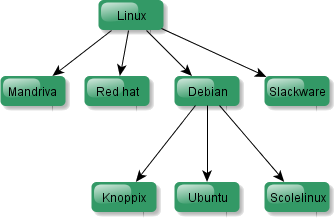
\includegraphics[height=2cm]{images/debian}
\end{center}
}%figues de la page de garde

\def\xxpied{%
Partie 1 -- Architecture matérielle et logicielle \\
Ch 2 : OS et Environnement de développement -- \xxactivite%
}

%---------------------------------------------------------------------------


\begin{document}
\chapterimage{png/Fond_Arch}
\pagestyle{empty}


%%%%%%%% PAGE DE GARDE COURS
\ifcours
\begin{tikzpicture}[remember picture,overlay]
\node at (current page.north west)
{\begin{tikzpicture}[remember picture,overlay]
\node[anchor=north west,inner sep=0pt] at (0,0) {\includegraphics[width=\paperwidth]{\thechapterimage}};
\draw[anchor=west] (-2cm,-8cm) node [line width=2pt,rounded corners=15pt,draw=ocre,fill=white,fill opacity=0.6,inner sep=40pt]{\strut\makebox[22cm]{}};
\draw[anchor=west] (1cm,-8cm) node {\huge\sffamily\bfseries\color{black} %
\begin{minipage}{1cm}
\rotatebox{90}{\LARGE\sffamily\textsc{\color{ocre}\textbf{\xxnumpartie}}}
\end{minipage} \hfill
\begin{minipage}[c]{14cm}
\begin{titrepartie}
\begin{flushright}
\renewcommand{\baselinestretch}{1.1} 
\Large\sffamily\textsc{\textbf{\xxpartie}}
\renewcommand{\baselinestretch}{1} 
\end{flushright}
\end{titrepartie}
\end{minipage} \hfill
\begin{minipage}[c]{3.5cm}
{\large\sffamily\textsc{\textbf{\color{ocre} \discipline}}}
\end{minipage} 
 };
\end{tikzpicture}};
\end{tikzpicture}


\begin{tikzpicture}[overlay]
\node[shape=rectangle, 
      rounded corners = .25 cm,
	  draw= ocre,
	  line width=2pt, 
	  fill = ocre!10,
	  minimum width  = 2.5cm,
	  minimum height = 3cm,] at (18cm,0) {};
\node at (17.7cm,0) {\rotatebox{90}{\textbf{\Large\color{ocre}{\classe}}}};
%{};
\end{tikzpicture}

\vspace{3.5cm}

\begin{tikzpicture}[remember picture,overlay]
\draw[anchor=west] (-2cm,-6cm) node {\huge\sffamily\bfseries\color{black} %
\begin{minipage}{2cm}
\begin{center}
\LARGE\sffamily\textsc{\color{ocre}\textbf{\xxactivite}}
\end{center}
\end{minipage} \hfill
\begin{minipage}[c]{15cm}
\begin{titrechapitre}
\renewcommand{\baselinestretch}{1.1} 
\Large\sffamily\textsc{\textbf{\xxnumchapitre}}

\Large\sffamily\textsc{\textbf{\xxchapitre}}
\vspace{.5cm}

\renewcommand{\baselinestretch}{1} 
\normalsize\normalfont
\xxcompetences
\end{titrechapitre}
\end{minipage}  };
\end{tikzpicture}
\vfill

\begin{flushright}
\begin{minipage}[c]{.3\linewidth}
\begin{center}
\xxfigures
\end{center}
\end{minipage}\hfill
\begin{minipage}[c]{.6\linewidth}
\startcontents
\printcontents{}{1}{}
\end{minipage}
\end{flushright}

\begin{tikzpicture}[remember picture,overlay]
\draw[anchor=west] (4.5cm,-.7cm) node {
\begin{minipage}[c]{.2\linewidth}
\begin{flushright}

\includegraphics[width=2cm]{png/logoCC}
\end{flushright}
\end{minipage}
\begin{minipage}[c]{.2\linewidth}
\textsl{\xxauteur} \\
\textsl{\classe}
\end{minipage}
 };
\end{tikzpicture}
\newpage
\pagestyle{fancy}

\newpage
\pagestyle{fancy}

\else
\fi


%%%%%%%% PAGE DE GARDE TD
\iftd
%\begin{tikzpicture}[remember picture,overlay]
%\node at (current page.north west)
%{\begin{tikzpicture}[remember picture,overlay]
%\draw[anchor=west] (-2cm,-3.25cm) node [line width=2pt,rounded corners=15pt,draw=ocre,fill=white,fill opacity=0.6,inner sep=40pt]{\strut\makebox[22cm]{}};
%\draw[anchor=west] (1cm,-3.25cm) node {\huge\sffamily\bfseries\color{black} %
%\begin{minipage}{1cm}
%\rotatebox{90}{\LARGE\sffamily\textsc{\color{ocre}\textbf{\xxnumpartie}}}
%\end{minipage} \hfill
%\begin{minipage}[c]{13.5cm}
%\begin{titrepartie}
%\begin{flushright}
%\renewcommand{\baselinestretch}{1.1} 
%\Large\sffamily\textsc{\textbf{\xxpartie}}
%\renewcommand{\baselinestretch}{1} 
%\end{flushright}
%\end{titrepartie}
%\end{minipage} \hfill
%\begin{minipage}[c]{3.5cm}
%{\large\sffamily\textsc{\textbf{\color{ocre} \discipline}}}
%\end{minipage} 
% };
%\end{tikzpicture}};
%\end{tikzpicture}

%%%%%%%%%% PAGE DE GARDE TD %%%%%%%%%%%%%%%
%\begin{tikzpicture}[overlay]
%\node[shape=rectangle, 
%      rounded corners = .25 cm,
%	  draw= ocre,
%	  line width=2pt, 
%	  fill = ocre!10,
%	  minimum width  = 2.5cm,
%	  minimum height = 2.5cm,] at (18.5cm,0) {};
%\node at (17.7cm,0) {\rotatebox{90}{\textbf{\Large\color{ocre}{\classe}}}};
%%{};
%\end{tikzpicture}

% PARTIE ET CHAPITRE
%\begin{tikzpicture}[remember picture,overlay]
%\draw[anchor=west] (-1cm,-2.1cm) node {\large\sffamily\bfseries\color{black} %
%\begin{minipage}[c]{15cm}
%\begin{flushleft}
%\xxnumchapitre \\
%\xxchapitre
%\end{flushleft}
%\end{minipage}  };
%\end{tikzpicture}

% Bandeau titre exo
\begin{tikzpicture}[remember picture,overlay]
\draw[anchor=west] (-2cm,-4cm) node {\huge\sffamily\bfseries\color{black} %
\begin{minipage}{5cm}
\begin{center}
\LARGE\sffamily\color{ocre}\textbf{\textsc{\xxactivite}}

\begin{center}
\xxfigures
\end{center}

\end{center}
\end{minipage} \hfill
\begin{minipage}[c]{12cm}
\begin{titrechapitre}
\renewcommand{\baselinestretch}{1.1} 
\large\sffamily\textbf{\textsc{\xxtitreexo}}

\small\sffamily{\textbf{\textit{\color{black!70}\xxsourceexo}}}
\vspace{.5cm}

\renewcommand{\baselinestretch}{1} 
\normalsize\normalfont
\xxcompetences
\end{titrechapitre}
\end{minipage}  };
\end{tikzpicture}
\else
\fi


%%%%%%%% PAGE DE GARDE FICHE
\iffiche
\begin{tikzpicture}[remember picture,overlay]
\node at (current page.north west)
{\begin{tikzpicture}[remember picture,overlay]
\draw[anchor=west] (-2cm,-3.25cm) node [line width=2pt,rounded corners=15pt,draw=ocre,fill=white,fill opacity=0.6,inner sep=40pt]{\strut\makebox[22cm]{}};
\draw[anchor=west] (1cm,-3.25cm) node {\huge\sffamily\bfseries\color{black} %
\begin{minipage}{1cm}
\rotatebox{90}{\LARGE\sffamily\textsc{\color{ocre}\textbf{\xxnumpartie}}}
\end{minipage} \hfill
\begin{minipage}[c]{14cm}
\begin{titrepartie}
\begin{flushright}
\renewcommand{\baselinestretch}{1.1} 
\large\sffamily\textsc{\textbf{\xxpartie} \\} 

\vspace{.2cm}

\normalsize\sffamily\textsc{\textbf{\xxnumchapitre -- \xxchapitre}}
\renewcommand{\baselinestretch}{1} 
\end{flushright}
\end{titrepartie}
\end{minipage} \hfill
\begin{minipage}[c]{3.5cm}
{\large\sffamily\textsc{\textbf{\color{ocre} \discipline}}}
\end{minipage} 
 };
\end{tikzpicture}};
\end{tikzpicture}


\begin{tikzpicture}[overlay]
\node[shape=rectangle, 
      rounded corners = .25 cm,
	  draw= ocre,
	  line width=2pt, 
	  fill = ocre!10,
	  minimum width  = 2.5cm,
	  minimum height = 2.5cm,] at (18.5cm,0.5cm) {};
%	  minimum height = 2.5cm,] at (18.5cm,0cm) {};
\node at (17.7cm,0.5) {\rotatebox{90}{\textsf{\textbf{\large\color{ocre}{\classe}}}}};
%{};
\end{tikzpicture}

\else
\fi






\section{Notion de système d'exploitation}

\subsection{Introduction}

Le système d'exploitation (\textit{Operating System -- OS}) est un programme chargé en mémoire vive dès le démarrage de l'ordinateur et qui reste en mémoire jusqu'à son extinction. 

Pour les \textbf{ordinateurs monoprocesseur} ce programme a pour but de donner l’illusion que l’ordinateur est multitâche lorsque plusieurs applications sont lancées en même temps. Pour cela, il stocke en mémoire les différentes applications que l’on veut exécuter. Il lance l’exécution d’une première application. Dès qu’il se produit une entrée-sortie ou, à défaut, lorsqu’un certain temps est écoulé (de l’ordre de la centaine de millisecondes), le noyau du système d’exploitation reprend la main et lance l’exécution d’une autre application. En pratique, le temps d’exécution d’une tâche dépasse rarement la dizaine de millisecondes.

Pour les \textbf{ordinateurs multiprocesseurs} ce programme a pour but de gérer les accés de chacun des processeurs à la mémoire et aux périphériques, ce qui permet
effectivement que l’ordinateur exécute plusieurs instructions à la fois. Les fabricants
de processeurs proposent même maintenant des processeurs qui contiennent en fait plusieurs
c\oe{}urs (dualcore, quadricore), c’est-à-dire que plusieurs processeurs (unité arithmétique
et logique et unité de contrôle) ont été regroupés sur un seul processeur.

Par ailleurs l'OS permet de manière générale de gérer l'organisation des données sur le disque dur ainsi que leur droit d'accès. Il gère aussi les différentes ressources et sert de garde-fou en cas de tentative de mauvaise utilisation des ressources de l'ordinateur.

Pour finir, l'OS permet à un ou plusieurs utilisateurs de s'identifier leur permettant ainsi d'utiliser un seul ordinateur sans nécessairement partager les données et les programmes. 


Il existe essentiellement deux grandes familles de systèmes d’exploitation. 

\begin{minipage}[c]{.7\linewidth}
Les systèmes d’exploitation de la famille Microsoft-Windows qui sont en situation de quasi-monopole sur les \textbf{ordinateurs personnels} (ils en équipent près de 90\%)

\end{minipage} \hfill
\begin{minipage}[c]{.25\linewidth}
\begin{center}

\includegraphics[width=.9\textwidth]{images/ms}
\end{center}
\end{minipage} 

\begin{minipage}[c]{.7\linewidth}
Les systèmes d’exploitation issus d’Unix (Mac OS X, iOS, GNU/Linux, Android, FreeBSD, NetBSD). Dans tous les domaines, sauf celui des ordinateurs personnels, les systèmes issus d’Unix sont majoritaires.  Linux s’est imposé comme un système universel puisqu’il équipe aussi bien les téléphones portables (Android) que les boîtiers prêtés par les fournisseurs d’accès à Internet, les ordinateurs personnels (Ubuntu/GNU Linux), les serveurs web et les supercalculateurs (plus de 90\% des calculateurs du TOP 500).

\end{minipage} \hfill
\begin{minipage}[c]{.25\linewidth}
\begin{center}

\includegraphics[width=.9\textwidth]{images/genlin}
\end{center}
\end{minipage} 

Il est possible d'installer plusieurs systèmes d'exploitation sur une même machine: double boot. Il est aussi possible d'émuler un système d'exploitation dans un autre système d'exploitation.

\subsection{Petit historique}

\begin{center}
\begin{tabular}{m{1cm}m{10cm}m{6cm}}
\textbf{1969} & 
Origines de UNIX. & 
\begin{center}
%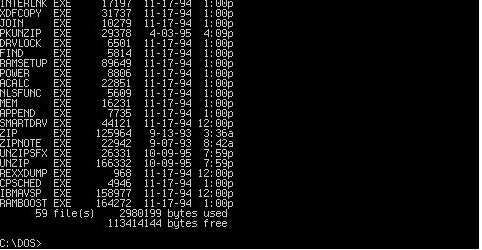
\includegraphics[width=7cm]{images/dos.jpg}
\end{center}
\end{tabular}

\begin{tabular}{m{1cm}m{10cm}m{6cm}}
\textbf{1984} & 
Sortie du premier OS de Microsoft : MS-DOS. & 
\begin{center}
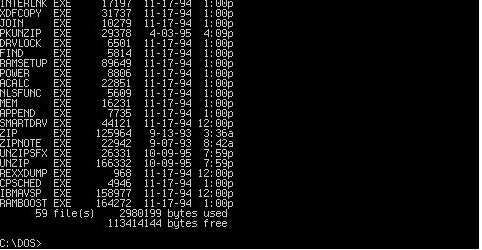
\includegraphics[width=6cm]{images/dos.jpg}
\end{center}
\end{tabular}

\begin{tabular}{m{1cm}m{10cm}m{6cm}}
\textbf{1984} & 
Richard Stallman\footnotemark[1] crée le projet GNU dans le but de développer un OS basé sur Unix, mais libre. & 
\begin{center}
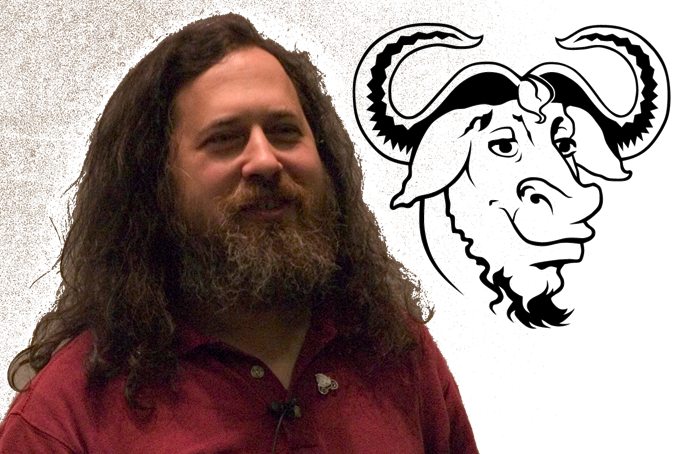
\includegraphics[width=6cm]{images/richard.png}
\end{center}
\end{tabular}

\begin{tabular}{m{1cm}m{10cm}m{6cm}}
\textbf{1991} & 

Linus Torvalds\footnotemark[2] entreprend de créer sur son temps libre son propre système d'exploitation. Ce système a pris le nom de Linux (contraction de Linus et Unix). Ce projet est complémentaire du projet GNU : tandis que Richard Stallman créait les programmes de base (programme de copie de fichier, de suppression de fichier, éditeur de texte), Linus s'est lancé dans la création du « cœur » d'un système d'exploitation : le noyau.
 & 
\begin{center}
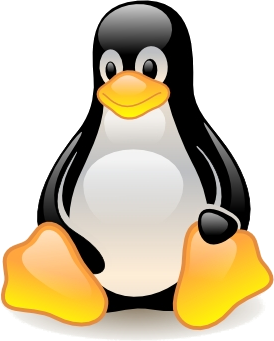
\includegraphics[width=3cm]{images/linux.png}
\end{center}
\end{tabular}

\end{center}

\footnotetext[1]{Chercheur en intelligence artificielle au MIT.}
\footnotetext[2]{\'Etudiant de l'Université de Helsinki (Finlande).}


%
%
%\begin{figure}[h]
%\begin{minipage}[c]{.49\linewidth}
%\begin{center}
%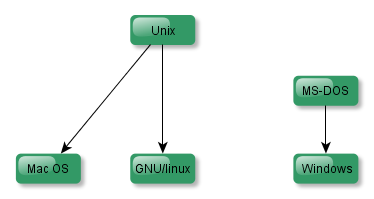
\includegraphics[width=.99\textwidth]{images/origine.png}
%\caption{Origine des systèmes d'exploitation}
%\label{}
%\label{essai1}
%\end{center}
%\end{minipage} \hfill
%\begin{minipage}[c]{.49\linewidth}
%Le projet GNU (programmes libres) et Linux (noyau d'OS) ont fusionné pour créer GNU/Linux.
%Théoriquement, on doit donc parler de GNU/Linux. C'est toutefois un peu difficile à écrire et prononcer, et par abus de langage, on dit souvent juste « Linux ». 
%\newline\newline
%Mac OS X est lui aussi basé sur Unix. En revanche, MS-DOS et Windows sont complètement à part.
%\end{minipage}
%\end{figure}
%




\begin{rem}
Un programme libre est un programme dont on peut avoir le code source, c'est-à-dire la « recette de fabrication ». Au contraire, Windows est un OS propriétaire dont le code source est conservé par Microsoft. On ne peut donc pas le modifier ou regarder comment il fonctionne à l'intérieur.

Un programme libre est donc la plupart du temps un programme gratuit. Mais c'est aussi un programme qu'on a le droit de copier, modifier, redistribuer. On dit aussi souvent que le programme est « Open Source » car son code source est ouvert ; tout le monde peut le voir.

Il existe quelques légères différences entre un programme « Open Source » et un programme « libre », mais nous n'entrerons pas dans les détails ici.
\end{rem}



\begin{rem}
\textit{Les distribution GNU/Linux}

Une distribution est un ensemble de logiciels articulés autour d'un noyau. GNU/Linux comprend un grand nombre de distributions. Elles diffèrent par la méthode d'installation, la gestion des programmes, la méthode pour installer des programmes. Attention, le terme distribution est différent du terme logiciel. De manière générale, un logiciel libre est installable sur n'importe quelle distribution. Dans le cas le plus défavorable, il sera nécessaire de \textbf{compiler} le logiciel.


%
%Pour simplifier la vie des utilisateurs et leur permettre de faire un choix, différentes distributions de Linux ont été créées. C'est un concept qui n'existe pas vraiment sous Windows. C'est un peu comme la différence entre Windows 7 Familial et Windows 7 Professionnel, mais cela va bien plus loin que ça.
%
%Voici ce qui peut différer d'une distribution à l'autre :
%\begin{itemize}
%\item l'installation : elle peut être très simplifiée comme très compliquée ;
%\item la gestion de l'installation des programmes. Si elle est bien faite et centralisée, elle peut rendre l'installation de nouveaux logiciels plus simple que sous Windows, comme nous le verrons plus loin !
%\item les programmes préinstallés sur l'ordinateur (Windows est par exemple livré avec Internet Explorer et Windows Media Player).
%\end{itemize}
%En fait, une distribution est en quelque sorte l'emballage de Linux. Le cœur, lui, reste le même sur toutes les distributions.
%
%Il existe un grand nombre de distributions Linux différentes:
%\begin{itemize}
%\item Slackware : une des plus anciennes distributions de Linux. Elle existe encore aujourd'hui !
%\item Mandriva : éditée par une entreprise française, elle se veut simple d'utilisation ;
%\item Red Hat : éditée par une entreprise américaine, cette distribution est célèbre et très répandue, notamment sur les serveurs ;
%\item SuSE : éditée par l'entreprise Novell ;
%\item Debian : la seule distribution qui soit gérée par des développeurs indépendants plutôt que par une entreprise. C'est une des distributions les plus populaires.
%\end{itemize}
%
%
%
%
%\begin{figure}[h]
%
%\begin{minipage}[c]{.49\linewidth}
%Prenons l'exemple de la distribution Debian.
%Les autres distributions sont gérées par des entreprises, ce qui ne les empêche pas d'être « Open Source » et gratuites, même si nous pouvons également les acheter pour avoir droit à une assistance (hotline…). Debian est donc la seule distribution éditée par des particuliers bénévoles à travers le monde. 
%Debian a tellement de succès que de nombreuses distributions sont basées sur Debian, ce sont donc des… distributions de distributions. 
%Ubuntu est une des distributions les plus populaires à l'heure actuelle.
%\end{minipage} \hfill
%\begin{minipage}[c]{.49\linewidth}

%\end{minipage}

%\begin{center}
%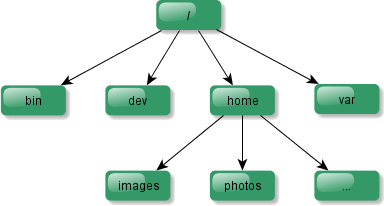
\includegraphics[width=.6\textwidth]{images/archilin.png}
%
%\textit{Différentes distributions GNU/Linux}
%
%\end{center}

\end{rem}




\subsection{À quoi ressemble Linux ?}


%\subsubsection{En mode console}

%\begin{figure}[h]
\begin{minipage}[c]{.49\linewidth}
Une des réticences à l'utilisation d'une distribution GNU/Linux est le mode console. 

Ce mode de fonctionnement peut paraître effrayant et peu accessible pour un utilisateur novice. Cependant, le mode console permet de faire une grande partie des opérations faisable avec la souris ce qui, avec l'expérience, améliore l'efficacité de l'utilisateur.
\end{minipage} \hfill
\begin{minipage}[c]{.49\linewidth}
\begin{center}
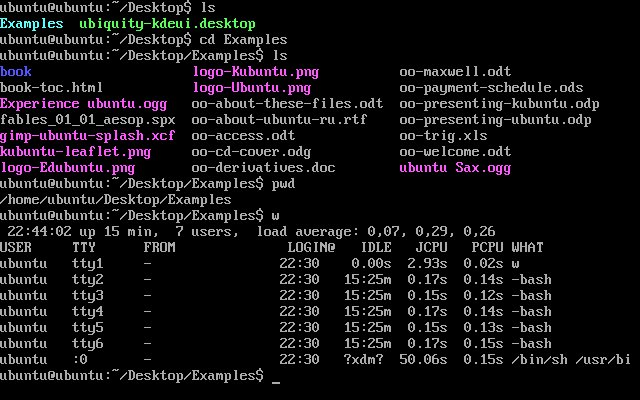
\includegraphics[width=.9\textwidth]{images/commande.jpg}
\end{center}
\end{minipage}
%
%\begin{warn}
%\textsc{ATTENTION}
%
%Ce serait une lourde erreur de croire que l'utilisation des interprètes de commandes en mode text  est
%dépassée. Leur usage demande certes plus de travail au départ que l'utilisation d'un shell
%graphique. Mais c'est l'une des façons les plus productives de faire exécuter des tâches à un
%ordinateur et pour l'administrateur d'un système, c'est bien souvent un outil indispensable.
%\end{warn}
%\end{minipage}
%\end{figure}

%\subsubsection{En mode graphique}

\vspace{.25cm}

Le mode graphique semble beaucoup plus accueillant pour quelqu'un venant de Windows. 
Il y a plusieurs modes graphiques, tous les modes graphiques sont basés sur un programme appelé X. On parle aussi de serveur d'affichage.

\begin{figure}[h]
\begin{minipage}[c]{.33\linewidth}
\begin{center}
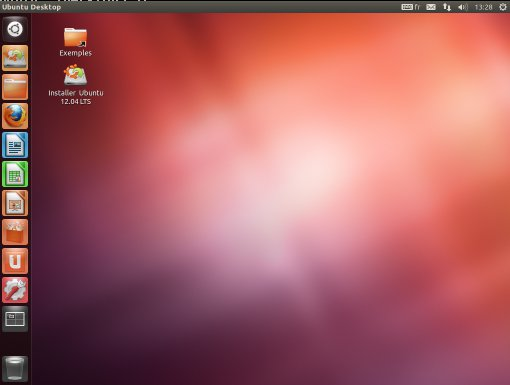
\includegraphics[height=3.5cm]{images/unity.jpg}

\textit{Ubuntu}
%\caption{Kbuntu}
%\label{}
%\label{essai1}
\end{center}
\end{minipage} \hfill
\begin{minipage}[c]{.33\linewidth}
\begin{center}
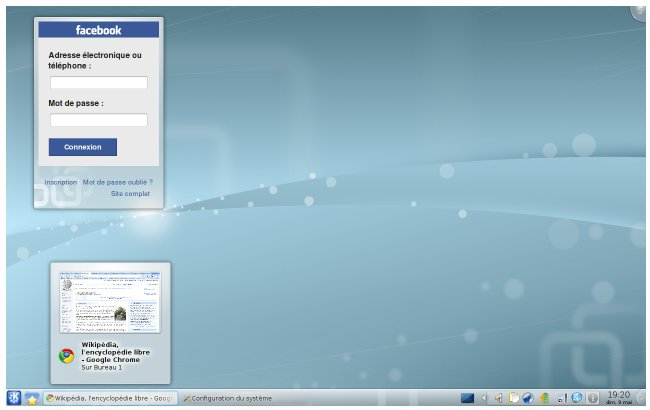
\includegraphics[height=3.5cm]{images/kbuntu.jpg}
%\caption{Kubuntu, basé sur KDE}

\textit{Kubuntu, basé sur KDE}
%\label{}
%\label{essai1}
\end{center}
\end{minipage} \hfill
\begin{minipage}[c]{.33\linewidth}

\begin{center}
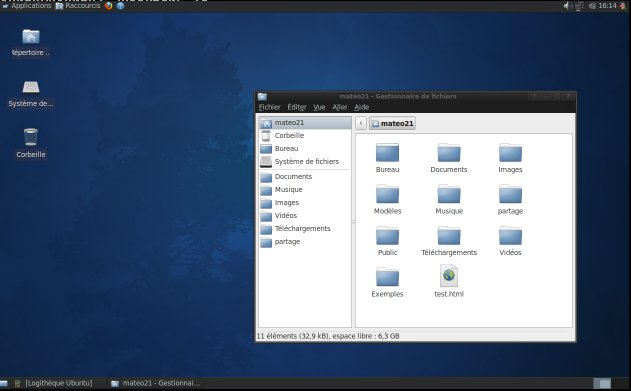
\includegraphics[height=3.5cm]{images/xbuntu.jpg}
%\caption{Xubuntu, basé sur XFCE}

\textit{Xubuntu, basé sur XFCE}
%\label{}
%\label{essai1}
\end{center}
\end{minipage} 
\end{figure}

\subsection{Identification des utilisateurs}

Les systèmes d'exploitation Unix comme Microsoft sont multi-utilisateur : chaque utilisateur
dispose d'un identifiant auprès du système (et en général, d’un mot de passe correspondant).

\begin{figure}[h]
\begin{minipage}[c]{.49\linewidth}
\begin{center}
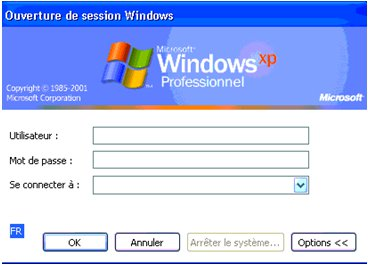
\includegraphics[height=5cm]{images/loginWin.jpg}

\textit{Fenêtre d'identification de Windows}
%\caption{Fenêtre d'identification de Windows}
%\label{}
\end{center}
\end{minipage} \hfill
\begin{minipage}[c]{.49\linewidth}
\begin{center}
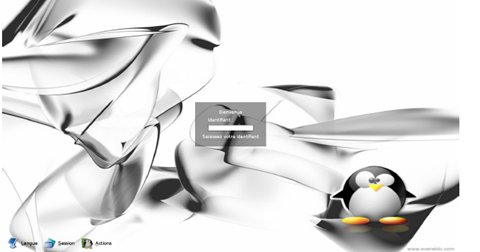
\includegraphics[height=5cm]{images/loginLin.jpg}

\textit{Fenêtre d'identification de Linux}
%\label{}
\end{center}
\end{minipage}
\end{figure}

%
%Vous disposez d'un compte Windows avec des droits d'utilisateur limités accessible depuis n’'importe quel ordinateur du lycée sur le réseau Pédagogique.
%\begin{itemize}
%\item login: prénom.nom
%\item mdp: date de naissance au format JJMMAAAA
%\end{itemize}
%
%Vous pouvez dès à présent changer votre mot de passe pour sécuriser l’accès à votre compte.
%
%
%Un compte utilisateur vous à été créé dans le système informatique, auquel est associé un identifiant,
%et un mot de passe. 
%De plus vous avez été déclaré comme
%étant membre d'un ou plusieurs groupes d'utilisateurs, ce qui va vous donner certains droits
%vis-à-vis du système informatique. 


%
%\subsection{Shell et interface graphique}
%
%Après avoir reconnu l'identifiant et le mot de passe comme valide le système
%d'exploitation lance un programme (ou un ensemble de programmes)
%qu'on appelle parfois shell. 
%Il existe aussi des shells en mode texte, on les appelle alors aussi interprètes de commandes :
%ce sont des programmes qui attendent une commande de l'utilisateur sous forme d'une
%ligne de texte, l'exécutent, attendent de nouveau une commande, l'exécutent, etc. Ils étaient
%historiquement utilisés sur des terminaux en mode texte, c'est-à-dire, une combinaison
%d’un clavier et d’un écran incapable d'afficher autre chose que du texte en orange sur fond
%noir (ou en vert sur fond noir). Aujourd'hui, ces terminaux ont quasiment disparu mais tous
%les systèmes Unix proposent des émulateurs de terminaux.
%
%
%\begin{figure}[h]
%\begin{minipage}[c]{.49\linewidth}
%
%Un tel émulateur est présenté
%ici. Les trois commandes pwd, ls et date on été tapé afin d'afficher le nom du répertoire de travail (print working directory), de lister son
%contenu et d'afficher la date et l'heure. Il a ensuite tapé une commande plus compliquée,
%qui permet en une ligne, certes complexe, de savoir combien de fichiers sont présents sur
%l'ordinateur (on peut lire à la suite la réponse de la machine).
%
%\end{minipage} \hfill
%\begin{minipage}[c]{.49\linewidth}
%\begin{center}
%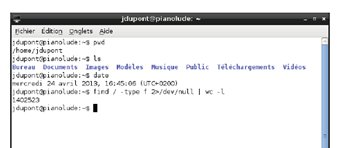
\includegraphics[width=.8\textwidth]{images/shell.jpg}
%\caption{Exemple de shell}
%\label{}
%\label{essai1}
%\end{center}
%\end{minipage}
%\end{figure}



\subsection{La structure des dossiers et fichiers}

Le nombre de fichiers étant généralement élevé, ils sont organisés en une structure arborescente
de répertoires. Du point de vue de l'utilisateur, un répertoire est un ensemble de fichiers et de sous répertoires, désignés par des noms.
%
%\begin{savoir}
%\textsc{SAVOIR-FAIRE Utiliser un système de fichiers}
%
%Dans un système de fichiers préexistant, il faut savoir :
%\begin{itemize}
%\item Se repérer dans l'arborescence. Cela demande de connaître dans les grandes
%lignes la structure du système de fichiers, de savoir retrouver
%son répertoire personnel et d'en connaître également l'organisation.
%\item Se déplacer dans cette arborescence, au moyen des fenêtres d'un shell graphique
%ou d'une commande (cd dans la plupart des systèmes d'exploitation). 
%\end{itemize}
%
%\end{savoir}

Du point de vue conceptuel, un fichier est une séquence finie d'octets, sans signification
a priori : c'est le programme qui lira cette séquence d'octets qui décidera de la façon de
la comprendre. Il peut contenir des données de tout type : texte, son, vidéo et même des
programmes directement exécutables par le processeur (programmes dits « binaires » ou
« en langage machine »).

Les fichiers présents sur le disque dur sont répertoriés dans une ou plusieurs tables, stockées
à un endroit du disque conventionnellement fixé, qui donnent des informations relatives
à ces fichiers, appelées métadonnées, notamment :
\begin{itemize}
\item date de création, de dernière modification, de dernière lecture;
\item taille du fichier;
\item emplacement des données du fichier sur le disque;
\item suivant les systèmes de fichiers employés, un numéro identifiant le fichier, appelé
inode sous Unix.
\end{itemize}

La table des métadonnées est aussi appelée table des inodes. Du point de vue du système d'exploitation, un répertoire est juste un fichier particulier,
qui contient une liste de couples $(n, i)$ où $n$ est un nom de fichier et $i$ l'inode du fichier.
Une information supplémentaire est stockée dans la table des inodes pour indiquer, pour
chaque fichier, s'il s'agit d'un fichier de données ordinaire ou d'un répertoire.


\subsubsection{La racine}

Dans un système de fichiers, il y a toujours ce qu'on appelle une racine, c'est-à-dire un gros dossier de base qui contient tous les autres dossiers et fichiers.

Sous Windows, il y a en fait plusieurs racines. \textit{C:\textbackslash} est la racine de votre disque dur, \textit{D:\textbackslash} est la racine de votre lecteur CD (par exemple).

Sous Linux, il n'y a qu'une et une seule racine : « / ». Il n'y a pas de lettre de lecteur car justement, Linux ne donne pas de nom aux lecteurs comme le fait Windows. Il dit juste « La base, c'est / ».

Il n'y a pas de dossier de plus haut niveau que /, c'est-à-dire qu'il n'existe pas de dossier qui contienne le dossier /. Quand on est à la racine, on ne peut pas remonter en arrière car… on est déjà tout au début.

\subsubsection{Architecture des dossiers}

Sous Windows, un dossier peut être représenté de la manière suivante : \textit{C:\textbackslash Program Files\textbackslash Gimp 2}. On dit que Gimp 2 est un sous-dossier du dossier Program Files, lui-même situé à la racine.

Vous noterez que c'est l'antislash \textbackslash (aussi appelé backslash) qui sert de séparateur aux noms de dossiers. Sous Linux, c'est au contraire le / (slash) qui sert de séparateur.
Il n'y a pas de \textit{C:} sous Linux, la racine (le début) s'appelant juste /.

Le dossier de notre superprogramme ressemblerait plutôt à quelque chose comme cela : \textit{/usr/bin/}. On dit que \textit{bin} est un sous-dossier du dossier \textit{usr}, lui-même situé à la racine.

\begin{figure}[h]
\begin{minipage}[c]{.49\linewidth}
\begin{center}
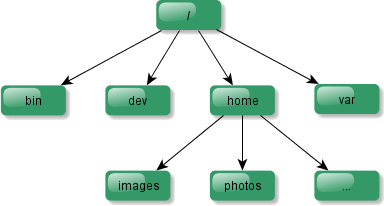
\includegraphics[width=.9\textwidth]{images/archilin.png}
\textit{Organisation des dossiers de Linux}
\end{center}
\end{minipage} \hfill
\begin{minipage}[c]{.49\linewidth}

Sous Windows, on a l'habitude de trouver souvent les mêmes dossiers à la racine : Documents and Settings, Program Files, Windows… Sous Linux, vous vous en doutez, les dossiers sont complètement différents. 
\newline\newline

Quelques dossiers courants sous linux:
\begin{itemize}
\item \textit{boot} : fichiers permettant le démarrage de Linux;
\item \textit{etc} : fichiers de configuration;
\item \textit{home} : répertoires personnels des utilisateurs. On en a déjà parlé un peu avant : c'est dans ce dossier que vous placerez vos fichiers personnels, à la manière du dossier Mes documents de Windows.
\end{itemize}
\end{minipage}
\end{figure}


\subsubsection{Quelques commandes classiques pour se déplacer dans l'arborescence:}

\begin{itemize}
\item \textit{pwd} : afficher le dossier actuel
\item \textit{ls} : lister les fichiers et dossiers
\item \textit{cd}: changer de dossier
\item \textit{du}: taille occupée par les dossiers
\item \textit{cp} : copier un fichier
\item \textit{mv} : déplacer un fichier
\item \textit{rm} : supprimer des fichiers et dossiers
\item \textit{mkdir} : créer un dossier
\end{itemize}


Ces quelques fonctions peuvent s'avérer nécessaires car elles sont utilisables dans Python pour manipuler les fichiers. 

%Utiliser le joker *

Le symbole * est appelé joker, ou encore wildcard en anglais sous Linux. 

\begin{minipage}[c]{.46\linewidth}
\begin{term}

Le joker vous permet de copier par exemple tous les fichiers image .jpg dans un sous-dossier :
\begin{termi}[h]
cp *.jpg mondossier/
\end{termi}
\end{term}
\end{minipage}\hfill
\begin{minipage}[c]{.46\linewidth}
\begin{term}
Vous pouvez aussi vous en servir pour copier tous les fichiers dont le nom commence par « so » :
\begin{termi}[h]
cp so* mondossier/
\end{termi}
\end{term}
\end{minipage}

\subsection{Droits d’accès}

Les droits d'accès font partie des propriétés d'un fichier. On peut recenser 3 principaux droits pour un fichier : 
\begin{itemize}
\item le droit en lecture (\textit{r -- read}), qui permet à l'utilisateur de lire le contenu du fichier;
\item le droit en écriture (\textit{w -- write}), qui permet à l'utilisateur d'écrire dans le fichier;
\item le droit d'exécution (\textit{x -- execute}), qui permet à l'utilisateur d'exécuter le fichier.
\end{itemize}

Par ailleurs pour un même ordinateur, il peut exister plusieurs utilisateurs. Ces utilisateurs peuvent de plus appartenir à un groupe.

Ainsi il est possible de distribuer des droits à un utilisateur, à un groupe d'utilisateurs ou à tous les utilisateurs.  

\begin{minipage}[c]{.45\linewidth}
\begin{center}
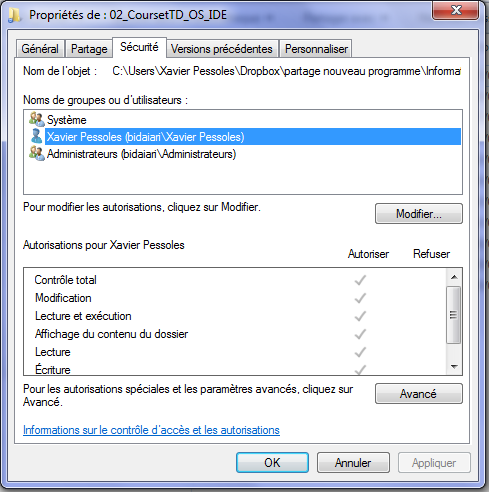
\includegraphics[width=.85\textwidth]{images/droits_win.png}
\end{center}
\end{minipage}\hfill
\begin{minipage}[c]{.45\linewidth}
\begin{center}
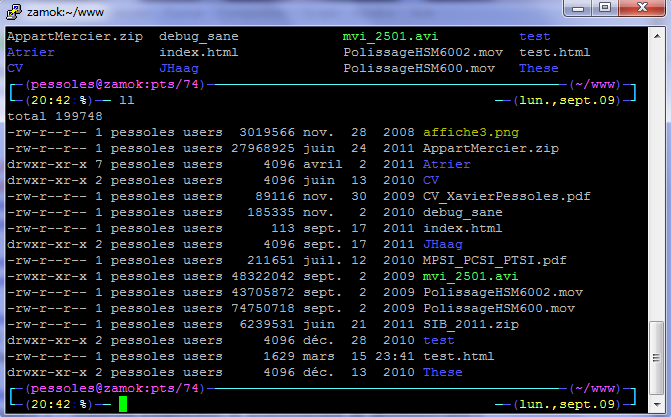
\includegraphics[width=.8\textwidth]{images/droits_lin.png}
$$
-\underbrace{rw-}_{1}\underbrace{r--}_{2}\underbrace{r--}_{3}
$$
\begin{itemize}
\item 1 : droits pour l'utilisateur pessoles;
\item 2 : droits pour l'utilisateur user;
\item 3 : droits pour le reste du monde.
\end{itemize}
\end{center}
\end{minipage}

%Vous êtes inscrit dans un groupe associé à la classe dans laquelle vous êtes. Vous avez accès en lecture/écriture dans Poste de travail/groupes au répertoires d'échanges de la classe. C'est données son stockées sur un serveur distant est accessible sur tous les ordinateur du lycée.

\begin{warn}
Toutes les données que ce soit dans votre espace personnel ou sur les serveurs du lycée ne sont stockées qu'a titre provisoire. Il vous appartient de faire des sauvegardes régulières.
\end{warn}


\begin{warn}
Tenter d'accéder aux données d'autrui est considéré comme une atteinte à la vie privée.
\end{warn}

%Chaque entrée de la table des inodes comporte, en plus des métadonnées déjà mentionnées,
%les droits d'accès accordés aux utilisateurs du système. Ces droits, appelés aussi permissions,
%précisent qui a le droit de faire quoi sur le fichier ou le répertoire concerné (lecture/écriture/exécution). Pour
%voir ces permissions, il suffit d'effectuer un clic droit dans le gestionnaire de fichiers sur
%le répertoire, de choisir « Propriétés » dans le menu contextuel qui apparaît alors, puis de
%cliquer sur l’onglet « Permissions ». 


%\subsection{Lancement d'applications}
%
%\begin{savoir}
%\textsc{SAVOIR-FAIRE Lancer des applications}
%
%Pour lancer une application (un programme), on dispose essentiellement de deux
%possibilités :
%\begin{itemize}
%\item Cliquer sur un bouton, un menu ou un fichier du shell graphique. Cette méthode
%est en général à réserver pour des tâches simples ; elle offre l’avantage d’être
%intuitive et donc utilisable même par des utilisateurs débutants.
%\item Taper une commande dans un shell en mode texte. Dès que l'on veut exprimer des
%commandes plus complexes, comme par exemple passer des arguments à un
%programme ou manipuler des fichiers en masse, cette méthode s'avère quasi
%incontournable. Son utilisation est plus ou moins facilitée selon le système
%d'exploitation que l'on utilise.
%\end{itemize}
%
%Une fois que le système a constaté que l'utilisateur avait le droit d'exécution sur le programme,
%il réserve un espace dans la mémoire vive de l'ordinateur pour stocker les instructions
%du programme ainsi que ses données. Il copie le contenu du fichier exécutable en
%mémoire.
%Celui-ci n'est qu'une suite de bits qui codent les instructions dans le langage du processeur
%(on dit que le programme est en langage machine), il peut donc les exécuter en effectuant
%un branchement vers les premières instructions du programme.
%
%Lorsqu'on clique sur le nom ou l'icône d'un fichier, le gestionnaire de fichiers commence
%par déterminer de quel type de fichier il s'agit. Suivant les systèmes, il peut s'appuyer sur
%diverses informations :
%\begin{itemize}
%\item Le nom du fichier et tout particulièrement son suffixe. Ainsi un fichier dont le nom se
%termine par .odt sera t-il identifié comme un fichier OpenDocument (le gestionnaire
%consulte pour cela une table qui associe un type de fichier à chaque suffixe connu).
%\item Le contenu du fichier.
%\item Le fait que l'utilisateur ait ou non le droit d’exécuter ce fichier.
%\item Sur certains systèmes (Mac OS X en particulier) : métadonnées associées au fichier
%donnant son type.
%\end{itemize}
%Puis, une fois le type déterminé, il consulte une table (commune à tout le système ou
%spécifique au gestionnaire de fichiers, commune à tous les utilisateurs ou spécifique à l'utilisateur)
%indiquant à quelle application est associé ce type de fichier. Il lance alors l'application,
%en lui fournissant pour argument (c'est-à-dire comme information supplémentaire)
%le nom du fichier à ouvrir. Là encore, la situation est exactement la même que si on avait
%tapé ooffice nomdufichier dans un shell en mode texte.
%\end{savoir}
%
%
%\begin{savoir}
%\textsc{SAVOIR-FAIRE Écrire un programme et le lancer}
%
%Tout utilisateur peut écrire ses propres programmes. Il existe pour cela essentiellement
%trois possibilités :
%\begin{itemize}
%\item Les écrire en langage machine. C'est une tâche ardue car le langage machine est un
%langage de bas niveau dans lequel il est difficile ou au minimum fastidieux
%d'implanter des idées un tant soit peu complexes.
%\item Utiliser un compilateur. Il s'agit d'un outil traduisant un programme écrit dans un
%langage évolué en un programme en langage machine. Plus précisément, dans
%le cas du langage C par exemple, on pourra ainsi, à partir d'un fichier contenant
%le texte d'un programme C (appelé par exemple hello.c), produire un
%programme en langage machine (appelé par exemple hello).
%\item Faire appel à un interpréteur d'un langage évolué. Un interpréteur est un programme
%exécutable qui va lire le texte d'un programme dans un langage évolué
%pour l'exécuter pas à pas, sans passer par la phase intermédiaire de compilation.
%La compilation demande donc un traitement préliminaire avant de pouvoir exécuter le
%programme que l'on a écrit, mais produit en général des applications efficaces. À l'inverse,
%on peut interpréter un programme immédiatement après l'avoir écrit, mais il aura tendance
%à s'exécuter moins rapidement. \textbf{C'est vers cette solution que l'on va s'orienter au départ.}
%
%\end{itemize}
%
%Le choix entre compilation et interprétation dépend très largement du langage dans lequel
%on programme : certains ne proposent qu'une seule des deux possibilités, d'autres laissent
%le choix. Il existe même des situations intermédiaires où un programme peut être compilé
%dans un langage qui est plus proche du langage machine mais qui doit encore être interprété
%(on parle de bytecode).
%\end{savoir}


\section{Python}


\begin{minipage}[c]{.79\linewidth}

Python est un langage de programmation, dont la première version est sortie en 1991. Créé par Guido van Rossum, il a voyagé du Macintosh de son créateur, qui travaillait à cette époque au Centrum voor Wiskunde en Informatica aux Pays-Bas, jusqu'à se voir associer une organisation à but non lucratif particulièrement dévouée, la Python Software Foundation, créée en 2001. Ce langage a été baptisé ainsi en hommage à la troupe de comiques les « Monty Python ».

\subsection{À quoi peut servir Python ?}
\end{minipage} \hfill
\begin{minipage}[c]{.2\linewidth}
\begin{center}

\includegraphics[width=.99\textwidth]{images/monty.jpg}
%\label{}
\end{center}
\end{minipage}




Python est un langage puissant, relativement facile à apprendre et riche en possibilités. Il est possible d'étendre ses fonctionnalités. On peut aussi appeler des bibliothèques qui aident le développeur à travailler. 

%Dès l'instant où vous l'installez sur votre ordinateur, vous disposez de nombreuses fonctionnalités intégrées au langage que nous allons découvrir tout au long de ce livre.
%Il est, en outre, très facile d'étendre les fonctionnalités existantes, comme nous allons le voir. Ainsi, il existe ce qu'on appelle des bibliothèques qui aident le développeur à travailler sur des projets particuliers. Plusieurs bibliothèques peuvent ainsi être installées pour, par exemple, développer des interfaces graphiques en Python.

Python permet :
\begin{itemize}
\item de réaliser de petits programmes très simples, appelés scripts, chargés d'une mission très précise sur votre ordinateur;
\item des programmes complets, comme des jeux, des suites bureautiques, des logiciels multimédias, des clients de messagerie…
\item des projets très complexes, comme des progiciels (ensemble de plusieurs logiciels pouvant fonctionner ensemble, principalement utilisés dans le monde professionnel).
\end{itemize}

Voici quelques-unes des fonctionnalités offertes par Python et ses bibliothèques :
\begin{itemize}
\item créer des interfaces graphiques ;
\item faire circuler des informations au travers d'un réseau ;
\item dialoguer d'une façon avancée avec votre système d'exploitation ;
\item ...
\end{itemize}

\subsection{ Un langage de programmation interprété}
Python est un langage de programmation interprété, c'est-à-dire comme on l'a spécifié au que les instructions que vous lui envoyez sont « transcrites » en langage machine au fur et à mesure de leur lecture. D'autres langages (comme le C / C++) sont appelés « langages compilés » car, avant de pouvoir les exécuter, un logiciel spécialisé se charge de transformer le code du programme en langage machine. On appelle cette étape la « compilation ». À chaque modification du code, il faut rappeler une étape de compilation.

Les avantages d'un langage interprété sont la simplicité (on ne passe pas par une étape de compilation avant d'exécuter son programme) et la portabilité (un langage tel que Python est censé fonctionner aussi bien sous Windows que sous Linux ou Mac OS, et on ne devrait avoir à effectuer aucun changement dans le code pour le passer d'un système à l'autre). Cela ne veut pas dire que les langages compilés ne sont pas portables, loin de là ! Mais on doit utiliser des compilateurs différents et, d'un système à l'autre, certaines instructions ne sont pas compatibles, voire se comportent différemment.

En contrepartie, un langage compilé se révélera bien plus rapide qu'un langage interprété (la traduction à la volée de votre programme ralentit l'exécution), bien que cette différence tende à se faire de moins en moins sentir au fil des améliorations. De plus, il faudra installer Python sur le système d'exploitation que vous utilisez pour que l'ordinateur puisse comprendre votre code.

\subsection{Différentes versions de Python}

Lors de la création de la Python Software Foundation, en 2001, et durant les années qui ont suivi, le langage Python est passé par une suite de versions que l'on a englobées dans l'appellation Python 2.x (2.3, 2.5, 2.6…). Depuis le 13 février 2009, la version 3.0.1 est disponible. Cette version casse la compatibilité ascendante qui prévalait lors des dernières versions.

%Installation à la maison : https://code.google.com/p/pythonxy/wiki/Downloads?tm=2






\begin{thebibliography}{2}
\bibitem{Tous}{Wack, Conchon, Courant, deFalco, Dowek, Filliatre, Gonnord, Informatique pour tous en classes préparatoires aux grandes écoles, éditions Eyrolles.}
\bibitem{zero}{Apprenez à programmer en Python \url{http://www.siteduzero.com/}.}
\end{thebibliography}
\end{document}


\newpage

\section{Environnement de développement intégré}



\begin{figure}[h]
\begin{minipage}[c]{.79\linewidth}
Afin de faciliter la programmation on va utiliser un environnement de développement intégré.
On appelle environnement de développement intégré (parfois abrégé IDE) un logiciel qui
permet à la fois :
\begin{itemize}
\item d'écrire des programmes dans un éditeur adapté au langage ;
\item d'exécuter les programmes que l'on a écrits ;
\item de corriger des erreurs (déboguer) dans ces programmes ;
\item éventuellement de consulter de la documentation.
\end{itemize}

Il existe de nombreux environnement: IDLE, Eclipse, Emacs ou Vim ...

Nous allons utiliser  Spyder, qui est fourni avec plusieurs
distributions de Python (WinPython ou Python(x,y) sous Windows, via le projet Mac-
Ports sous MacOS, et enfin il existe des paquets pour la plupart des distributions Linux).

\textbf{Démarrer pythonxy puis dans la fenêtre ci-contre cliquer sur Spyder.}


\end{minipage} \hfill
\begin{minipage}[c]{.2\linewidth}

\begin{center}
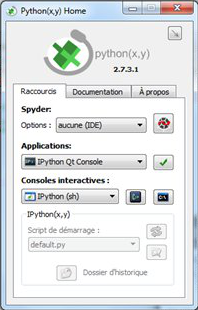
\includegraphics[width=.99\textwidth]{images/int1.png}
\label{}
\end{center}
\end{minipage}
\end{figure}

\begin{figure}[h]
\begin{minipage}[c]{.49\linewidth}

La fenêtre de Spyder est divisée en trois parties :
\begin{itemize}
\item L'éditeur à gauche, dans lequel on écrira les programmes.
\item L'explorateur en haut à droite, que nous utiliserons essentiellement comme débogueur,
mais qui peut également servir de documentation.
\end{itemize}
La console interactive en bas à droite, dans laquelle s'exécuteront les programmes.
\end{minipage} \hfill
\begin{minipage}[c]{.49\linewidth}
\begin{center}
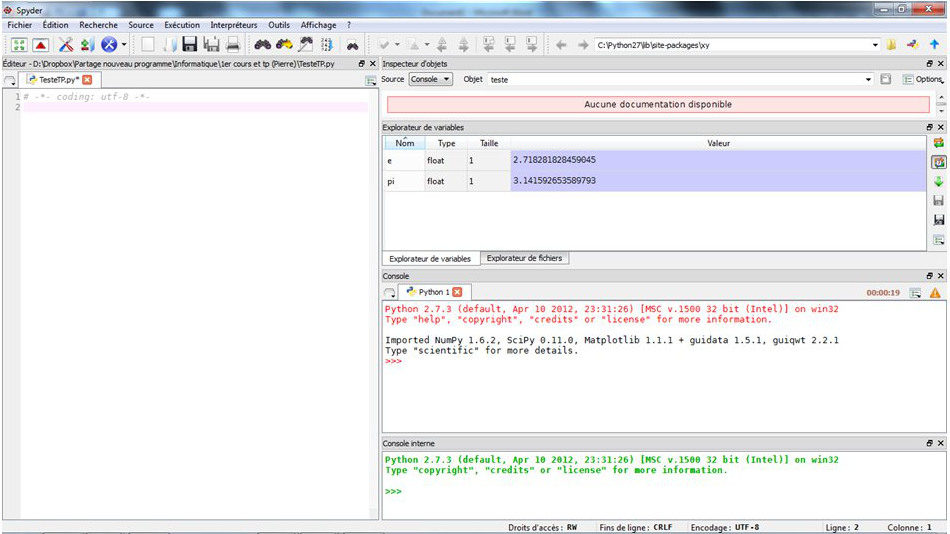
\includegraphics[width=.9\textwidth]{images/fen.png}
\label{}
\end{center}
\end{minipage}
\end{figure}

\subsection{La console interactive}


\begin{figure}[h]
\begin{minipage}[c]{.69\linewidth}

Aller dans "interpréteurs" puis démarrer un interpréteur Ipython (cf figure ci-contre).
\newline\newline
In [1]:
La dernière ligne, qui commence par In suivi d’un nombre entre crochets, attend que l’on
tape une commande : c’est le mode interactif de Python, où chaque ligne tapée est immédiatement
exécutée. Ainsi, si l’on tape une expression, sa valeur s’affiche.

\end{minipage} \hfill
\begin{minipage}[c]{.3\linewidth}
\begin{center}
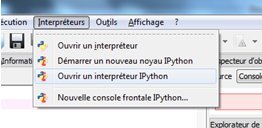
\includegraphics[width=.99\textwidth]{images/fen2.jpg}
\label{}
\end{center}
\end{minipage}
\end{figure}


\begin{py}
\begin{python}[h]
In [1]: 2+2
Out[1]: 4
\end{python}
\end{py}




On appelle session de travail une suite d’instructions tapées dans une fenêtre Python interactive
avec les réponses correspondantes. Il est possible d’enregistrer le contenu d’une
session de travail à l’aide de la commande Enregistrer l’historique... accessible par un clic
droit dans la console.


\begin{figure}[h]
\begin{minipage}[c]{.49\linewidth}
Dans ce mode, on peut d’ores et déjà utiliser des variables pour stocker des valeurs. L’affectation
s’écrit avec le symbole = et n’affiche aucune valeur ; mais la variable mémorise la
valeur qu’on lui a donnée et peut être utilisée dans la suite de la session.
\end{minipage} \hfill
\begin{minipage}[c]{.49\linewidth}
\begin{py}
\begin{python}[h]
In [2]: a=2
In [3]: a+a
Out[3]: 4
\end{python}
\end{py}
\end{minipage}
\end{figure}









\begin{figure}[h]
\begin{minipage}[c]{.49\linewidth}
Notons que si l’on utilise dans une expression une variable à laquelle on n'a jamais donné
de valeur, une erreur se produit.
\end{minipage} \hfill
\begin{minipage}[c]{.49\linewidth}
\begin{py}
\begin{python}[h]
In [4]: b+1

Traceback (most recent call last):
File "<ipython console>", line 1, in <module>
NameError: name 'b' is not defined
\end{python}
\end{py}

\end{minipage}
\end{figure}




\begin{rem}

\textsc{Lien avec le shell}

IPython peut également être utilisé comme un terminal système de remplacement. Son comportement par défaut est très familier aux shell Unix.

\begin{py}
\begin{python}[h]
In [1]: pwd
Out[1]: u'C:\\Python27\\lib\\site-packages\\xy'

In [2]: cd ..
C:\\Python27\\lib\\site-packages

In [3]: pwd
Out[3]: u'C:\\Python27\\lib\\site-packages'

In [4]: ls
 Le volume dans le lecteur C s'appelle OS
 Le numéro de série du volume est A65E-3C0C

 Répertoire de C:\\Python27\\lib\\site-packages

01/08/2013  11:11    <REP>          .
01/08/2013  11:11    <REP>          ..
04/05/2013  15:40    <REP>          _markerlib
10/11/2008  19:40            11776  _memimporter.pyd
...
\end{python}
\end{py}

\end{rem}

Enfin il est possible de rappeler une ligne tapée précédemment à l’aide des flèches « haut »
et « bas », et de modifier cette ligne avant de relancer son calcul avec « Entrée ».

À chaque nouvelle session, les valeurs des variables sont perdues ; les instructions précédemment
tapées peuvent toujours être rappelées, mais cela reste peu pratique et on n’imagine
évidemment pas écrire un programme complet de la sorte. Les sessions interactives
sont donc à réserver pour tester très rapidement l’évaluation de quelques expressions que
l’on ne souhaite pas conserver par la suite.

\subsection{L'éditeur}

\begin{figure}[h]
\begin{minipage}[c]{.49\linewidth}
Dès que l’on veut écrire un programme, ou même tout simplement une suite d'instructions
dont on veut garder une trace, on utilise l'éditeur.
\newline\newline \textbf{Écrivons dans celui-ci un premier programme Python.}
\end{minipage} \hfill
\begin{minipage}[c]{.49\linewidth}
\begin{py}
\begin{python}[h]
print("Bonjour !")
x = 42
print(x)
\end{python}
\end{py}
\end{minipage}
\end{figure}

On observe déjà plusieurs différences par rapport au mode interactif :
\begin{itemize}
\item les mots-clés du langage (comme print) et les nombres se colorent pour ressortir sur le
reste du texte.
\item Les chaînes de caractères (entre guillemets) se colorent également.
\item Lorsque l'on tape une parenthèse ouvrante, la parenthèse fermante correspondante se
crée automatiquement ; et lorsque l'on place le curseur à droite d'une parenthèse, celle-ci
se colore en rouge s'il manque la parenthèse correspondante, en vert sinon.
\end{itemize}

Pour que la machine exécute (on dit aussi interprète) les instructions que l’on a tapées,
il faut le lui demander par la commande Exécution du menu du même nom (raccourci
clavier F5). Les instructions sont alors lues et exécutées, et le résultat, lorsqu’il
y en a un, s'affiche dans l'interpréteur interactif.

\begin{savoir}
\textsc{SAVOIR-FAIRE Utiliser un environnement de développement intégré}

Le minimum pour pouvoir utiliser un environnement de développement intégré est
de savoir :
\begin{itemize}
\item Lancer l’IDE
\item Ouvrir et enregistrer les programmes que l’on écrit
\item Exécuter ces programmes
\end{itemize}
\end{savoir}

\subsection{Le débogueur}

La fenêtre située en haut à droite de Spyder possède plusieurs onglets :
\begin{itemize}
\item Inspecteur d'objets permet d'obtenir de l'aide sur un type ou sur une fonction ;
\item Explorateur de variables permet de connaître la valeur de toutes les variables à tout moment
;
\item Explorateur de fichiers permet de parcourir les fichiers Python du système de fichiers.
\end{itemize}


\begin{figure}[h]
\begin{minipage}[c]{.49\linewidth}
Pour chercher une erreur dans un programme, ou tout simplement pour mieux comprendre
son fonctionnement, il peut être utile de l'exécuter pas à pas. Si cela reste faisable de tête
pour des programmes simples, il devient vite beaucoup plus commode de confier cette
tâche à la machine. Voyons comment procéder sur l'exemple ci-contre.
\end{minipage} \hfill
\begin{minipage}[c]{.49\linewidth}
\begin{py}
\begin{python}[h]
x = 10
y = 7
x = x+y
y = x
x = 5 / (x-y)
\end{python}
\end{py}

\end{minipage}
\end{figure}




Après avoir recopié ce programme dans l'éditeur, au lieu de l'exécuter normalement, on
appelle la commande Déboguer du menu Exécution (raccourci Ctrl+F5 ). La première
ligne du programme que l'on a écrit (x=10) est surlignée et recopiée dans l'interpréteur, mais
elle n'est pas encore exécutée : on peut le vérifier en constatant que x n'a pas la valeur 10
dans l'explorateur de variables. 

Pour exécuter cette ligne, on peut cliquer sur le bouton Pas
en avant , ou bien taper n (comme next) dans l'interpréteur. La ligne est alors exécutée, x
prend la valeur 10, et c'est la ligne suivante (y=7) qui est surlignée. On peut ensuite continuer
à exécuter les lignes les unes après les autres et surveiller l'évolution des différentes variables
dans l'explorateur.

Comme il peut être malcommode de devoir cliquer sur un bouton pour chaque ligne du
programme alors que seules certaines posent problème, on peut fixer des points d'arrêts dans
le programme. Pour cela, on se place sur la ligne à laquelle on désire faire une pause dans
l'exécution du programme, et on choisit Ajouter un point d'arrêt dans le menu Exécution
(raccourci F12). On peut également double-cliquer dans la marge gauche du programme ;
un symbole s'affiche alors en face de cette ligne. Par exemple, dans le programme ci-avant,
il peut être judicieux de placer un point d'arrêt à la dernière ligne, dans laquelle risque de
se produire une division par zéro.

Désormais, si au lieu d'effectuer un Pas en avant, on choisit Continuer ( ou c dans l'interpréteur
interactif), le programme s'exécute normalement jusqu'au prochain point d'arrêt,
puis attend une commande de l'utilisateur pour continuer à s'exécuter. Dans cet exemple,
on voit dans l'explorateur de variables que x et y contiennent toutes deux la valeur 17 et qu'il
y aura donc effectivement une division par zéro.

\begin{savoir}
\textsc{SAVOIR-FAIRE Utiliser un débogueur}
Pour corriger une erreur dans un programme,
\begin{itemize}
\item on détermine les variables qui ne se comportent pas comme prévu
\item on localise l'erreur au moyen d'une exécution pas à pas
\end{itemize}
Dans le cas d'un programme de taille trop importante pour une exécution pas à pas
complète, on veillera à placer des points d'arrêt aux endroits critiques, c'est-à-dire les
opérations arithmétiques pouvant produire des erreurs, les fins de boucles, certains
tests...
\end{savoir}



\begin{exercice}
\textsc{Exercice } Cet exercice a pour seul but de s'entraîner à manipuler l'environnement de développement
intégré, il n'est pas nécessaire de savoir déjà programmer en Python pour le réaliser.
\begin{itemize}
\item Taper le programme suivant dans l'éditeur et l'exécuter. Que se passe-t-il ?
\begin{py}
\begin{python}[h]
i = 10
while i != 0 :
i = 1-i
print(i)
\end{python}
\end{py}
(Il est possible qu'à ce stade il soit nécessaire de fermer complètement l’IDE et de le rouvrir pour
continuer...)
\item Exécuter ce programme pas à pas et observer les valeurs successives prises par la variable i. \item Expliquer
le comportement observé à la première question.
\item Placer un point d'arrêt à un endroit approprié du programme pour montrer son comportement
sans avoir besoin de détailler des étapes inutiles.
\end{itemize}
\end{exercice}


















